%% --------------------------------------------------------------------
%% thesis.tex -- MAIN FILE 
%% --------------------------------------------------------------------

%-----<<<<<<<<<<<< START >>>>>>>>>>>>-----
\documentclass [a4paper,12pt]{report}  
\usepackage[a-2u]{pdfx}      		
\usepackage{lmodern}
\usepackage[T1]{fontenc}
\usepackage{textcomp}
\usepackage[USenglish]{babel}
\usepackage{epigraph}
\usepackage{bm}
\usepackage{dsfont}
\usepackage{longtable}
\usepackage{rotating} % rotating tables using sidewaystable
\usepackage{afterpage} % keeping related figures and plots on the same page
\usepackage{tikz} % plotting the neural network
\usetikzlibrary{positioning}
\usepackage{hyperref}

\usepackage{adjustbox}
\usepackage{array}

\newcolumntype{R}[2]{%
	>{\adjustbox{angle=#1,lap=\width-(#2)}\bgroup}%
	l%
	<{\egroup}%
}

\newcommand*\rot{\multicolumn{1}{R{45}{1em}}} % command for rotating column headers in tabular
\renewcommand{\vec}[1]{\bm{#1}}
\newcommand{\norm}[1]{\left\lVert#1\right\rVert}

%-----<<<<<<<<<<<< DEFINITIONS >>>>>>>>>>>>----- 
\def \BookName {Master's thesis}
\def \Bookname {Can Machines Explain Stock Returns?}
\def \BooknameCZ {Mohou stroje vysv\v{e}tlit akciov\'{e} v\'{y}nosy?} 
\def \AutorDP {Bc.\ Karol\'{i}na Chalupov\'{a}}													
\def \AuthorDP {Karolina Chalupova} 						%English characters
\def \FirstNameDP {Karolina} 				
\def \LastNameDP {Chalupova} 							
\def \Email {chalupova.karolina@gmail.com}
\def \Year {2020}
\def \Place {Prague}
\def \Subject {Can Machines Explain Stock Returns?}
\def \Keywords {(interpretable) machine learning, neural networks, stock returns}
\def \Klic {
	(interpretovateln\'{e}) strojov\'{e} u\v{c}en\'{i}, 
	neuronov\'{e} s\'{i}t\v{e}, 
	akciov\'{e} v\'{y}nosy
} 					
\def \JEL {
	\href{http://ideas.repec.org/j/C45.html}{C45},			%http://www.aeaweb.org/journal/elclasjn_hold.html
 	\href{http://ideas.repec.org/j/G12.html}{G12}
}	
\def \Thesisweb {\href{https://github.com/KarolinaChalupova/DiplomaThesis}}		%thesis webpage
\def \AcademicYear {2019/2020}
\def \Supervisor {doc.\ PhDr.\ Jozef Barun\'{i}k, Ph.D.}
\def \Consultant {Mgr. Martin Hronec}
\def \StudyProgram {Economics and Finance}
\def \EmailSup {barunik@fsv.cuni.cz}
\def \EmailCon {martin.hronec@fsv.cuni.cz}
\def \CUNI {Charles University}
\def \FSS {Faculty of Social Sciences}
\def \IES {Institute of Economic Studies}

%-----<<< METADATA >>>-----
%filecontents must be in form of text, do not put definition reference like ``\AuthorDP'' inside
%\usepackage{filecontents}
%\begin{filecontents*}{Thesis.xmpdata}
%		\Author{Firstname Lastname} 
%		\Title{The Price Elasticity of Gasoline Demand: A Meta-Analysis}
%		\Keywords{keywordone, keywordtwo, keywordthree, keywordfour}
%		\Subject{Price Elasticity of Gasoline Demand}
%		\Publisher{Charles University} 
%\end{filecontents*} 

%-----<<<<<<<<<<<< STYLES >>>>>>>>>>>>-----      														
\usepackage{Styles/Head}
\usepackage{Styles/Mystyle}	

%-----<<<<<<<<<<<< DOCUMENT >>>>>>>>>>>>-----
\begin{document}
	\frontmatter                   							%lowercase roman pagination for front matter
	\clubpenalty 9999 										%not so many orphants
	\widowpenalty 9999 										%not so many widows
	
	%-----<<< HEAD >>>-----
	\pagestyle{empty}                       				%no visible pagination here                    
	\BookHead
	%-----<<< ---- >>>-----
	
	%-----<<< DECLARATION >>>-----
	\vfill

\vglue 14cm

\section*{Declaration of Authorship}
The author hereby declares that he or she compiled this thesis independently, using only the listed resources and literature, and the thesis has not been used to obtain any other academic title.

\bigskip 

\noindent The author grants to Charles University permission to reproduce and to distribute copies of this thesis in whole or in part and agrees with the thesis being used for study and scientific purposes.
\vspace{0.5cm}

\begin{table}[!hbp]
\begin{tabular}{lr}
\hspace{-0.3cm} Prague, \today
\hspace{3cm}       
 \begin{tabular}{p{4.5cm}}
    \vspace{0.6cm} \\
     \hline \\ 
		\vspace{-0.7cm} \hspace{0.6cm} \AuthorDP
 \end{tabular}

\end{tabular}
\end{table}
        					%input file
	\clearpage
	%-----<<< ----------- >>>-----
	
	
	%-----<<< ABSTRACT >>>-----
	\phantomsection											%bookmark anchor
	\pdfbookmark[0]{Abstract}{abst}        	 				%add bookmark
	\section*{Abstract}

The abstract should concisely summarize the
contents of a thesis. Since potential readers should be able to
make their decision on the personal relevance based on the abstract,
the abstract should clearly tell the reader what information
he can expect to find in the thesis. The most essential issue
is the problem statement and the actual contribution of described
work. The authors should always keep in mind that the
abstract is the most frequently read part of a thesis. It should
contain at least 70 and at most 120 words (200 when you are writing a thesis).
Do not cite anyone in the abstract.

\bigskip

\begin{tabular}{lp{8.6cm}}
		\textbf{JEL Classification} & \JEL \\
		\textbf{Keywords} & \Keywords \\
 		& \\
		\textbf{Title} & \Bookname \\
 		\textbf{Author's e-mail} & \texttt{\href{mailto:\Email}{\Email}}\\
		\textbf{Supervisor's e-mail} & \texttt{\href{mailto:\EmailSup}{\EmailSup}}\\
\end{tabular}

\bigskip

\section*{Abstrakt}\label{abstract}

TODO cesky preklad abstraktu. 

\bigskip

\begin{tabular}{lp{7.7cm}}
		\textbf{Klasifikace JEL} & \JEL \\
		\textbf{Kl\'{i}\v{c}ov\'{a} slova} & \Klic \\
 		& \\
		\textbf{N\'{a}zev pr\'{a}ce} & \BooknameCZ \\
 		\textbf{E-mail autora} & \texttt{\href{mailto:\Email}{\Email}}\\
		\textbf{E-mail vedouc\'{i}ho pr\'{a}ce} & \texttt{\href{mailto:\EmailSup}{\EmailSup}}\\
\end{tabular}

       					%input file
	\clearpage
	%-----<<< -------- >>>-----
	
	%-----<<< ACKNOWLEDGMENTS >>>-----
	\section*{Acknowledgments}
The author is especially grateful to PhDr. Jozef Barun\'{i}k, Ph.D., as well as Mgr. Martin Hronec for guiding, inspiring and offering valuable critics to her work both in the big picture and the technical details, always pointing to the right direction. The author is once again thankful to Mgr. Martin Hronec and his colleague MPhil. Ond\v{r}ej Tobek, Ph.D, for sharing their meticulously cleaned dataset. The author would also like to thank Bc. Tom\'{a}\v{s} Turl\'{i}k for drawing her attention to an important detail in data cleaning. A further thank you extends to RNDr. Milan Straka, Ph.D., for his outstanding courses in machine learning and advising this thesis on hyperparameter tuning in Python. This thesis is part of a project that has received funding from the European Union’s Horizon 2020 research and innovation programme under the Marie Skłodowska-Curie grant agreement No. 681228. Any mistakes are, of course, the author's own. 


\vfill

\noindent Typeset in \LaTeX  using the \href{https://is.cuni.cz/studium/eng/predmety/index.php?do=predmet&kod=JEM001}{IES Thesis Template}. 

\bigskip

\noindent \textbf{Bibliographic Record} \\
\LastNameDP, \FirstNameDP: \emph{\Bookname}. \BookName. \CUNI, \FSS, \IES, \Place. \Year, pages \ref*{TotPages}. Advisor: \Supervisor


      					%input file
	\clearpage
	%-----<<< --------------- >>>-----
	
	%-----<<< TABLE OF CONTENTS >>>-----
	\pagestyle{fancy} 										%headers style
	\fancyhead[LO]{\sffamily Contents}			 			%headers in sans serif and not in uppercase
	\phantomsection											%bookmark anchor
	\pdfbookmark[0]{Contents}{toc}        	 				%add bookmark
	\tableofcontents
	\label{toc}
	\clearpage
	%-----<<< ----------------- >>>-----
	
	%-----<<< LIST OF TABLES >>>-----
	\fancyhead[LO]{\sffamily List of Tables}				%headers in sans serif and not in uppercase
	\phantomsection											%bookmark anchor
	\addcontentsline{toc}{chapter}{List of Tables}			%add LofT to the Table of Contents
	\listoftables
	\clearpage
	%-----<<< --------------- >>>-----
	
	%-----<<< LIST OF FIGURES >>>-----  
	\fancyhead[LO]{\sffamily List of Figures}
	\phantomsection											%bookmark anchor
	\addcontentsline{toc}{chapter}{List of Figures}			%add LofF to the Table of Contents
	\listoffigures
	\clearpage
	%-----<<< ---------------- >>>-----
	
	%-----<<< ACRONYMS >>>-----   
	\fancyhead[LO]{\sffamily Acronyms}
	\phantomsection											%bookmark anchor
	\addcontentsline{toc}{chapter}{Acronyms}				%add Acronyms to the Table of Contents
	\chapter*{Acronyms}

\begin{acronym}[OFDI]
{\setlength{\baselineskip}%
{0.67\baselineskip}

\acro{ML}{Machine Learning}
\acro{CAPM}{Capital Asset Pricing Model}

\par}
\end{acronym}							%List of Acronyms
	\clearpage
	%-----<<< ---------------- >>>-----
	
		%-----<<< NOTATION >>>-----   
	\fancyhead[LO]{\sffamily Notation}
	\phantomsection											%bookmark anchor
	\addcontentsline{toc}{chapter}{Notation}				%add Acronyms to the Table of Contents
	\chapter*{Notation}

The following mathematical symbols are used throughout the thesis. 

Scalars (integer or real), vectors, and matrices are denoted using italics, for example:

$$
a, \vec{a}, \vec{A}
$$

for scalar, vector and matrix respectively. An element of a vector $\vec{a}$ is denoted as

$$
a_i
$$

and an element of a matrix $\vec{A}$ is denoted as 

$$
a_{i,j}.
$$

Random variables are denote using uppercase regular font, for example:

$$
A
$$ 

and they always represent a scalar random variable.  



							%List of Acronyms
	\clearpage
	%-----<<< ---------------- >>>-----
	
	%-----<<< THESIS PROPOSAL >>>----- 
	\fancyhead[LO]{\sffamily Master's Thesis Proposal}
	\phantomsection											%bookmark anchor
	\addcontentsline{toc}{chapter}{Thesis Proposal}			%add Proposal to the Table of Contents
	\chapter*{Master's Thesis Proposal}

\begin{tabular}{lp{10.1cm}}
		\hline
		\textbf{Author} &\href{mailto:\Email}{\AutorDP}\\
		\textbf{Supervisor} &\href{mailto:\EmailSup}{\Supervisor}\\
		\textbf{Proposed topic} &\Bookname\\
		\hline
\end{tabular}

\bigskip

\small
\paragraph{Motivation}


\paragraph{Hypotheses}


\paragraph{Methodology}


\paragraph{Expected Contribution}


\paragraph{Outline}


\paragraph{Core bibliography}




\vfill
\begin{table}[!hbp]
\begin{tabular}{lr}

 \begin{tabular}{p{3.5cm}}
     \hline \hspace{1cm} Author
 \end{tabular}
 
 \hspace{5.5cm}
 
 \begin{tabular}{p{3.5cm}}
     \hline \hspace{0.8cm} Supervisor
 \end{tabular}

 
 \end{tabular}
 \end{table}

\normalsize





							%Thesis proposal
	\clearpage
	%-----<<< ---------------- >>>-----
	
	%-----<<< MAIN MATTER >>>-----
	\mainmatter                   							%start arabic pagination from 1
	\autohdr												%automatic headers for main matter
	\chapter{Introduction}
\label{chap:int}

The question of what explains differences in stock returns between firms has been consuming the academia for over five decades now. The question is interesting from an economist's perspective: putting a price tag on uncertain future payoffs of stocks reflects human impatience and attitudes to risk \citep{cochrane2009asset} and with them, human behavioral biases \citep{kahneman2013prospect}. Stock returns also speak of the complex web of relations between firms: as companies form relationships, they become exposed to similar risks, and their returns correlate \citep{chi2010network}. Thus, studying the cross-section of stock returns is an opportunity to understand human behavior as well as macro-phenomena that emerge in the network of firm's relationships.

The academia has accumulated hundreds of variables that are proposed to explain stock returns. From a statistician's viewpoint, the determinants of stock returns are notoriously over-studied, which brings along the issues of publication bias and multiple hypothesis testing, leading to many false discoveries. \cite{harvey2016and} and \cite{mclean2016does} have famously shown that "most claimed research findings in financial economics are likely false" \cite[p.~5]{harvey2016and} and the field entered a deep crisis. The multidimensional challenge \citep{cochrane2011presidential} emerged: which of the published and unpublished determinants of stock returns are valid, and which are erroneous? What is the wheat, and what is the chaff among stock return predictors?

At the same time, machine learning (ML) drives scientific discovery, progress in many industries and influences human lives day-to-day. Machines don't just play chess and go, drive cars, translate text and recognize images, all better than humans. They are used in basic research in chemistry, and in applied research in medical diagnostics. Machines even do art. [TODO add references to all]. 

Finance is no exception: here as well, ML is gaining popularity both in the academia and the industry. Neural networks in particular beat traditional modeling approaches (such as regression and discriminant analysis) in many financial areas, such as bankruptcy prediction, bank failure prediction, credit rating, bond rating, bond price forecasting, inflation forecasting, and, most often, stock returns prediction \citep{fadlalla2001analysis}. To cite just two more recent examples concerning stock returns: \cite{bryzgalova2019forest} are able to construct discount factor using random trees, overcoming major obstacles with the traditional portfolio-sorts methodology used in finance. \cite{gu2020empirical} and \cite{tobek2020does} show that neural networks used for stock return predictions are 2 to 4 times more profitable in terms of Sharpe ratio than traditional regression approaches.  

However, ML methods, neural networks in particular, are quite complex models and it is therefore challenging to interpret them and explain their decisions. At the same time, interpretability is crucial for many reasons. The first reason is ethical: crudely speaking, we need to know why the auto-driven car did not see the cyclist, why we are not eligible for a loan, and why we are loosing money in the stock market. Sometimes, we even have a \textit{right} to know the explanation to an algorithmic decision, as acknowledged by new European legislation [TODO add citation]. A second reason is practical: it is difficult to improve a model without a deep understanding of how it makes particular decisions. For example, using feature importance measures, one can uncover which inputs to the model are important, and use this knowledge to limit the amount of noise in the model and add stronger predictors \citep{de2018advances}. This brings a need for interpretable, or explainable, ML, now a quickly developing field \citep{molnar2020interpretable}. In other words, as the machine-learning approaches are becoming the norm in the applied field, a need arises to understand the models on a deeper level – which brings us back to the economic underpinnings of stock returns.

It is quite well established that neural networks are the best-performing model to predict stock returns  \citep{gu2020empirical}. However, interpretation of the networks in this domain is yet in its infancy \citep{gu2020empirical}. This thesis aims to fill this gap. It offers three contributions for both academic and applied finance. First, it uncovers which variables the networks consider important for predicting stock returns. Financial constraints, behavioral biases of investors and risk of illiquidity are the groups that appear as most important. This builds on existing findings of \cite{gu2020empirical} and \cite{tobek2020does} while making them more interpretable and precise, by using a measure that is well-grounded in theory and has an interesting and ready interpretation, and by offering detailed decompositions of the results across time, model architectures and ensemble sub-models. Second, this thesis is likely the first work to extract the \textit{sign} of the effect that the predictors have on the predicted returns in neural networks -- it is exciting to see that the direction overwhelmingly agrees with the economic motivations of the predictors. Third, by developing a novel metric of feature importance, Portfolio Reliance, the thesis is in all likelihood the first to point out which variables drive the network's outstanding performance in forming long-short portfolios (predicting the winners and the losers among the stocks). 

Thus, modeling stock returns is viewed from multiple perspectives: the economic one, which strives to understand how investors and firms interact in the supply and demand for information, the statistical one, seeing the gamut of publications and their biases, that of an ML engineer, who sees the problem as making a prediction from noisy data full of complex interactions, and that of a finance practitioner, who strives to identify the future winners and losers in the market. This thesis attempts to bring the four approaches together. I uses use machine learning models to predict stock returns and then interpret them to bring us closer to the answers to the economists' questions. Finally, a finance practitioner can use the now more intelligible model, of which she understands the weaknesses and sources of performance.

The dataset is a liquid universe of globally traded stocks, from 1990 to 2018, and offers 30 stock-level variables that are a distillation of the last 50 years of research in the field. The performance of the networks in this thesis is at par with the state-of-the-art models for stock return prediction, which further enhances its relevance for financial practice. The thesis studies 4 feed-forward neural networks, consisting of 1 to 4 hidden layers. This architecture is ubiquitous in many financial applications \cite{fadlalla2001analysis}, which makes the work quite relevant also to other areas than stock return prediction.    

The thesis is structured as follows: Chaper \ref{chap:lit} offers a review of existing literature, focusing first on the economic motivation of stock return predictors, then on the current state of interpretable ML in stock returns, and finally on the selection of a suitable feature importance measure. Chapter \ref{chap:met} first describes the dataset and then explains the methodology behind training, evaluating and interpreting the networks used. Chapter \ref{chap:res} gives the results, first demonstrating the predictive ability and profitability of the networks, and then diving into their interpretation. Chapter \ref{con} concludes and offers areas for further research. 
              		%input field
	\chapter{Literature Review}
\label{chap:lit} 
	
 	
 	The field of asset pricing strives to put a value, or a price tag, on uncertain future payoffs. 
 	
 	One of the most studied problems in finance is explaining why different assets earn different returns. The problem is so central that an entire field evolved to solve it – the asset pricing. 
 	
 	
 	Answering this question is vital, as by doing so, one also explains many crucial phenomena. Why do some stock prices rise, while other stocks become worthless? What drives the returns - is it exposure to risk, market imperfections, mispricing or random chance? Is it all of them? Are some of the drivers more important than others? Is a given stock priced fairly, or is it too expensive or too cheap? How does the stock market go up and down? Why does it go mostly up? Why do some stocks go up in bad times? Are returns predictable? To what degree? Why do stock market bubbles occur? The answer to the over-arching problem of why different assets earn different returns would also explain all of these questions.  
 	
 	The question is so important that the in
 	
 	Asset pricing theory gives the following theoretical answer. Return of stock 
 	
 	\begin{equation}
 	r_t = \beta_{t-1}F_t + \epsilon_t  = g(C_{t-1})F_t + \epsilon_t \label{eq:asset_pricing}
 	\end{equation}
 	
 	The canonical answer to this question is that expected return of an asset at time $t$ is a linear function of systematic sources of risk, so-called factors ($F_t$). $\beta_{t-1}$, also called factor loadings, sensitivity to factors, or just betas, denote the amount of exposure to the underlying sources of risk: 
		
		\begin{equation}
			r_t = \beta_{t-1}F_t + \epsilon_t  = g(C_{t-1})F_t + \epsilon_t \label{eq:asset_pricing}
		\end{equation}
		
	
	
	
	$\beta_{t-1}$ is a $N \times K$ matrix, where $N$ denotes the number of assets and $K$ the amount of risk factors. $F_t$ is a $K \times1 $ vector.
	
	An important implication of \ref{eq:asset_pricing} is that the factor loadings, in turn, are a possibly non-linear function of firm-level characteristics ($C_{t-1}$). 
		
		\begin{equation}
			\beta_{t-1}= g(C_{t-1})\label{eq:characteristics_as_proxies}
		\end{equation}
	
	In the words of \cite{fama1993common}: "(...) if assets are priced rationally, variables that are
	related to average returns, such as size and book-to-market equity, must proxy for
	sensitivity to common (shared and thus undiversiable) risk factors in returns." 	
	
	The theoretical answer is therefore clear: the differences in average returns are explained by different exposure to risk factors. 
	Take the simplest example, the CAPM model, where $K=1$ and $F_t$ is a (scalar) return of market portfolio at time $t$ \citep{cochrane2009asset}: on average, a high return on a stock is just a compensation for the stock's high correlation $\beta_{t-1}$ with the market. 
	
	The empirical answer, however, is complicated. One empirical issue with estimating equation \ref{eq:asset_pricing} is that both $F_t$ and $\beta_{t-1}$ are unobservable \citep{kelly2019characteristics}. The question reduces to: how to obtain the factors? 
	
	The first approach is to use prior knowledge of empirical behavior of average returns to pre-specify factors $F_t$, treat them as known and observable and then estimate $\beta_{t-1}$. In the portfolio-sorting method, a characteristic is chosen (somehow). Stocks are then sorted into portfolios based on their value of this characteristic \citep{fama1993common}. It is then studied whether different returns of these portfolios can be explained by a simpler factor model, such as CAPM. Using this mehod, academia has generated about 300 factors \citep{harvey2016and}, considering the top journals only.
	
	\cite{bryzgalova2019forest} generalize the portfolio-sorts using random trees.     
	
	The second strand of literature treats both $F_t$ and $\beta_{t-1}$ as unobservable, and estimates them both from the data, using the  relationship that firm-level characteristics are proxies of factor loadings (\ref{eq:characteristics_as_proxies}). For example, \cite{kelly2019characteristics} use characteristics as instrumental variables for factor loadings. Once loadings are instrumented, they use them to estimate the corresponding factors. 
	
    
	
	

	
	   
	
	   
	




	\chapter{Data and Methodology}
\label{chap:met}

\section{Data}

	I obtain the dataset from \cite{tobek2020does}. The dataset comprises of liquid publicly traded shares from developed countries of Europe, Japan and Asia-Pacific (Australia, New Zealand, Hong Kong, and Singapore). The data is monthly and spans from 1990 to 2018. I use the liquid universe, which contains 8,350 companies,  totaling 1,607,117 observations. 
	
	This thesis uses 30 anomalies that were identified as strongest predictors of equity returns in the \cite{tobek2020does} paper. The authors compute 153  anomalies, firm-level characteristics that have been put forward by leading financial and accounting journals as predictors of equity returns. The authors then use the 153 anomalies in a single model, which allows individual effects to crowd each other out, and results in ordering of the predictors from the strongest to the weakest. This thesis takes 30 predictors identified as strongest on liquid global universe of stocks (Figure 8 in \cite{tobek2020does}).
	
	Table [TODO add summary table] shows the 30 anomalies studied. 
	
	I preprocess all predictors in the following manner (in line with \cite{gu2020empirical}). First, I winsorize bottom and top 1\% of each variable to mitigate the impact of observations with implausibly large or small values. Second, I center each variable so that its mean is 0 and subsequently normalize so that the resulting values lie between -1 and 1. This is done because neural networks work better with data on the same scale. Finally, I impute missing values by mean (that is, 0), as all values entering a neural network must be numerical and the value 0 can be interpreted as "no information". I perform all these operations on data grouped by year, that is, first split the data into groups by year, then apply the transformations and finally combine back into single dataset. The main motivation for this is to prevent information from getting from test sets to training and validation sets.    	
	
	Table \ref{tab:descr} shows descriptive statistics of the anomalies data after these transformations.
		
	Figure \ref{fig:corrplot}, shows plot of the correlation matrix of the anomalies.

	The task is to predict the return of given stock in month $t+1$ given that stock's anomalies as of the time $t$. (Two technical notes: first, the dataset is organized so that this shift is taken care of, i.e., the features corresponding to the given target have the same index. Second, the anomalies as of the time $t-1$ can be (and often are) calculated from raw data based on several preceding time periods, e.g., $t$, $t-1$, $t-2$ and therefore the time index  represents the entire information set rather than financial or accounting information being \textit{published} at that time index. For example, a single observation at a given time index $t$ consists of the target (stock's return in $t+1$), and anomalies calculated as of $t$, such as average return in the last six months ($t$, $t-1$, $t-2$, $t-3$, $t-4$, $t-5$))
	
	Figure \ref{fig:hist_returns} shows histogram of the targets (monthly returns). 
	
	
	

	%\begin{tabular}{lrrrrrrrr}
\toprule
{} &      count &  mean &     std &     min &     25\% &     50\% &     75\% &    max \\
\midrule
Lagged Momentum                            &  1607088.0 &   0.0 &  0.0316 & -0.1518 & -0.0053 & -0.0009 &  0.0029 &  1.000 \\
Seasonality                                &  1607088.0 &  -0.0 &  0.0282 & -0.2622 & -0.0034 & -0.0002 &  0.0021 &  1.000 \\
Short-Term Reversal                        &  1607088.0 &  -0.0 &  0.2430 & -0.9831 & -0.1276 & -0.0178 &  0.1027 &  1.000 \\
Momentum-Reversal                          &  1607088.0 &   0.0 &  0.0200 & -0.0802 & -0.0054 & -0.0008 &  0.0029 &  1.000 \\
52-Week High                               &  1607088.0 &  -0.0 &  0.3316 & -1.0000 & -0.1828 &  0.0764 &  0.2445 &  0.678 \\
RD / Market Equity                         &  1607088.0 &  -0.0 &  0.0169 & -0.0311 & -0.0001 &  0.0000 &  0.0000 &  1.000 \\
Liquidity Shocks                           &  1607088.0 &  -0.0 &  0.0055 & -0.0016 & -0.0001 & -0.0001 & -0.0000 &  1.000 \\
Earnings Predictability                    &  1607088.0 &   0.0 &  0.0158 & -0.0081 & -0.0006 &  0.0000 &  0.0000 &  1.000 \\
Seasonality 6-10 A                         &  1607088.0 &  -0.0 &  0.0220 & -0.1208 & -0.0055 &  0.0000 &  0.0029 &  1.000 \\
Change in Common Equity                    &  1607088.0 &  -0.0 &  0.0153 & -0.0199 & -0.0013 & -0.0003 & -0.0001 &  1.000 \\
Seasonality 6-10 N                         &  1607088.0 &   0.0 &  0.0220 & -0.1307 & -0.0050 &  0.0000 &  0.0020 &  1.000 \\
Seasonality 2-5 N                          &  1607088.0 &   0.0 &  0.0219 & -0.1313 & -0.0061 & -0.0005 &  0.0035 &  1.000 \\
Seasonality 2-5 A                          &  1607088.0 &  -0.0 &  0.0180 & -0.1002 & -0.0042 & -0.0000 &  0.0027 &  1.000 \\
Leverage Component of Book/Price           &  1607088.0 &   0.0 &  0.0089 & -0.0057 & -0.0002 & -0.0001 & -0.0000 &  1.000 \\
Amihud's Measure (Illiquidity)             &  1607088.0 &   0.0 &  0.0221 & -0.0113 & -0.0005 & -0.0002 & -0.0001 &  1.000 \\
Profit Margin                              &  1607088.0 &   0.0 &  0.0652 & -1.0000 & -0.0000 &  0.0011 &  0.0097 &  1.000 \\
Volume Trend                               &  1607088.0 &   0.0 &  0.2040 & -0.8532 & -0.0873 &  0.0000 &  0.0979 &  1.000 \\
Coefficient of Variation of Share Turnover &  1607088.0 &  -0.0 &  0.1144 & -0.1469 & -0.0625 & -0.0279 &  0.0170 &  1.000 \\
Earnings Forecast-to-Price                 &  1607088.0 &   0.0 &  0.0137 & -0.1066 & -0.0006 &  0.0000 &  0.0000 &  1.000 \\
Duration of Equity                         &  1607088.0 &   0.0 &  0.0624 & -1.0000 & -0.0006 &  0.0000 &  0.0068 &  1.000 \\
Seasonality 11-15 N                        &  1607088.0 &   0.0 &  0.0213 & -0.1246 & -0.0032 &  0.0000 &  0.0005 &  1.000 \\
Operating Profits to Assets                &  1607088.0 &   0.0 &  0.0562 & -0.3581 & -0.0122 &  0.0000 &  0.0011 &  1.000 \\
Max                                        &  1607088.0 &   0.0 &  0.1913 & -0.2571 & -0.1111 & -0.0544 &  0.0416 &  1.000 \\
Whited-Wu Index                            &  1607088.0 &   0.0 &  0.1681 & -0.7012 & -0.0528 &  0.0000 &  0.0489 &  1.000 \\
Net Operating Assets                       &  1607088.0 &  -0.0 &  0.0171 & -0.0869 & -0.0007 & -0.0001 &  0.0000 &  1.000 \\
Accruals                                   &  1607088.0 &   0.0 &  0.0484 & -0.3996 & -0.0043 &  0.0000 &  0.0033 &  1.000 \\
Idiosyncratic Risk                         &  1607088.0 &  -0.0 &  0.1999 & -0.2929 & -0.1204 & -0.0539 &  0.0528 &  1.000 \\
Coskewness                                 &  1607088.0 &  -0.0 &  0.1996 & -1.0000 & -0.1014 &  0.0000 &  0.1074 &  1.000 \\
Liquidity Beta 5                           &  1607088.0 &  -0.0 &  0.0724 & -0.3288 & -0.0298 &  0.0000 &  0.0213 &  1.000 \\
Liquidity Beta 3                           &  1607088.0 &  -0.0 &  0.0568 & -0.3347 & -0.0100 &  0.0000 &  0.0204 &  1.000 \\
\bottomrule
\end{tabular}

	
	\begin{table}
		\resizebox{\textwidth}{!}{\begin{tabular}{lrrrrrrrr}
\toprule
{} &      count &  mean &     std &     min &     25\% &     50\% &     75\% &    max \\
\midrule
Lagged Momentum                            &  1607088.0 &   0.0 &  0.0316 & -0.1518 & -0.0053 & -0.0009 &  0.0029 &  1.000 \\
Seasonality                                &  1607088.0 &  -0.0 &  0.0282 & -0.2622 & -0.0034 & -0.0002 &  0.0021 &  1.000 \\
Short-Term Reversal                        &  1607088.0 &  -0.0 &  0.2430 & -0.9831 & -0.1276 & -0.0178 &  0.1027 &  1.000 \\
Momentum-Reversal                          &  1607088.0 &   0.0 &  0.0200 & -0.0802 & -0.0054 & -0.0008 &  0.0029 &  1.000 \\
52-Week High                               &  1607088.0 &  -0.0 &  0.3316 & -1.0000 & -0.1828 &  0.0764 &  0.2445 &  0.678 \\
RD / Market Equity                         &  1607088.0 &  -0.0 &  0.0169 & -0.0311 & -0.0001 &  0.0000 &  0.0000 &  1.000 \\
Liquidity Shocks                           &  1607088.0 &  -0.0 &  0.0055 & -0.0016 & -0.0001 & -0.0001 & -0.0000 &  1.000 \\
Earnings Predictability                    &  1607088.0 &   0.0 &  0.0158 & -0.0081 & -0.0006 &  0.0000 &  0.0000 &  1.000 \\
Seasonality 6-10 A                         &  1607088.0 &  -0.0 &  0.0220 & -0.1208 & -0.0055 &  0.0000 &  0.0029 &  1.000 \\
Change in Common Equity                    &  1607088.0 &  -0.0 &  0.0153 & -0.0199 & -0.0013 & -0.0003 & -0.0001 &  1.000 \\
Seasonality 6-10 N                         &  1607088.0 &   0.0 &  0.0220 & -0.1307 & -0.0050 &  0.0000 &  0.0020 &  1.000 \\
Seasonality 2-5 N                          &  1607088.0 &   0.0 &  0.0219 & -0.1313 & -0.0061 & -0.0005 &  0.0035 &  1.000 \\
Seasonality 2-5 A                          &  1607088.0 &  -0.0 &  0.0180 & -0.1002 & -0.0042 & -0.0000 &  0.0027 &  1.000 \\
Leverage Component of Book/Price           &  1607088.0 &   0.0 &  0.0089 & -0.0057 & -0.0002 & -0.0001 & -0.0000 &  1.000 \\
Amihud's Measure (Illiquidity)             &  1607088.0 &   0.0 &  0.0221 & -0.0113 & -0.0005 & -0.0002 & -0.0001 &  1.000 \\
Profit Margin                              &  1607088.0 &   0.0 &  0.0652 & -1.0000 & -0.0000 &  0.0011 &  0.0097 &  1.000 \\
Volume Trend                               &  1607088.0 &   0.0 &  0.2040 & -0.8532 & -0.0873 &  0.0000 &  0.0979 &  1.000 \\
Coefficient of Variation of Share Turnover &  1607088.0 &  -0.0 &  0.1144 & -0.1469 & -0.0625 & -0.0279 &  0.0170 &  1.000 \\
Earnings Forecast-to-Price                 &  1607088.0 &   0.0 &  0.0137 & -0.1066 & -0.0006 &  0.0000 &  0.0000 &  1.000 \\
Duration of Equity                         &  1607088.0 &   0.0 &  0.0624 & -1.0000 & -0.0006 &  0.0000 &  0.0068 &  1.000 \\
Seasonality 11-15 N                        &  1607088.0 &   0.0 &  0.0213 & -0.1246 & -0.0032 &  0.0000 &  0.0005 &  1.000 \\
Operating Profits to Assets                &  1607088.0 &   0.0 &  0.0562 & -0.3581 & -0.0122 &  0.0000 &  0.0011 &  1.000 \\
Max                                        &  1607088.0 &   0.0 &  0.1913 & -0.2571 & -0.1111 & -0.0544 &  0.0416 &  1.000 \\
Whited-Wu Index                            &  1607088.0 &   0.0 &  0.1681 & -0.7012 & -0.0528 &  0.0000 &  0.0489 &  1.000 \\
Net Operating Assets                       &  1607088.0 &  -0.0 &  0.0171 & -0.0869 & -0.0007 & -0.0001 &  0.0000 &  1.000 \\
Accruals                                   &  1607088.0 &   0.0 &  0.0484 & -0.3996 & -0.0043 &  0.0000 &  0.0033 &  1.000 \\
Idiosyncratic Risk                         &  1607088.0 &  -0.0 &  0.1999 & -0.2929 & -0.1204 & -0.0539 &  0.0528 &  1.000 \\
Coskewness                                 &  1607088.0 &  -0.0 &  0.1996 & -1.0000 & -0.1014 &  0.0000 &  0.1074 &  1.000 \\
Liquidity Beta 5                           &  1607088.0 &  -0.0 &  0.0724 & -0.3288 & -0.0298 &  0.0000 &  0.0213 &  1.000 \\
Liquidity Beta 3                           &  1607088.0 &  -0.0 &  0.0568 & -0.3347 & -0.0100 &  0.0000 &  0.0204 &  1.000 \\
\bottomrule
\end{tabular}
}
		\caption{Descriptive Statistics of the Anomalies}
		\label{tab:descr}
	\end{table}


	\begin{center}
		\begin{figure}
			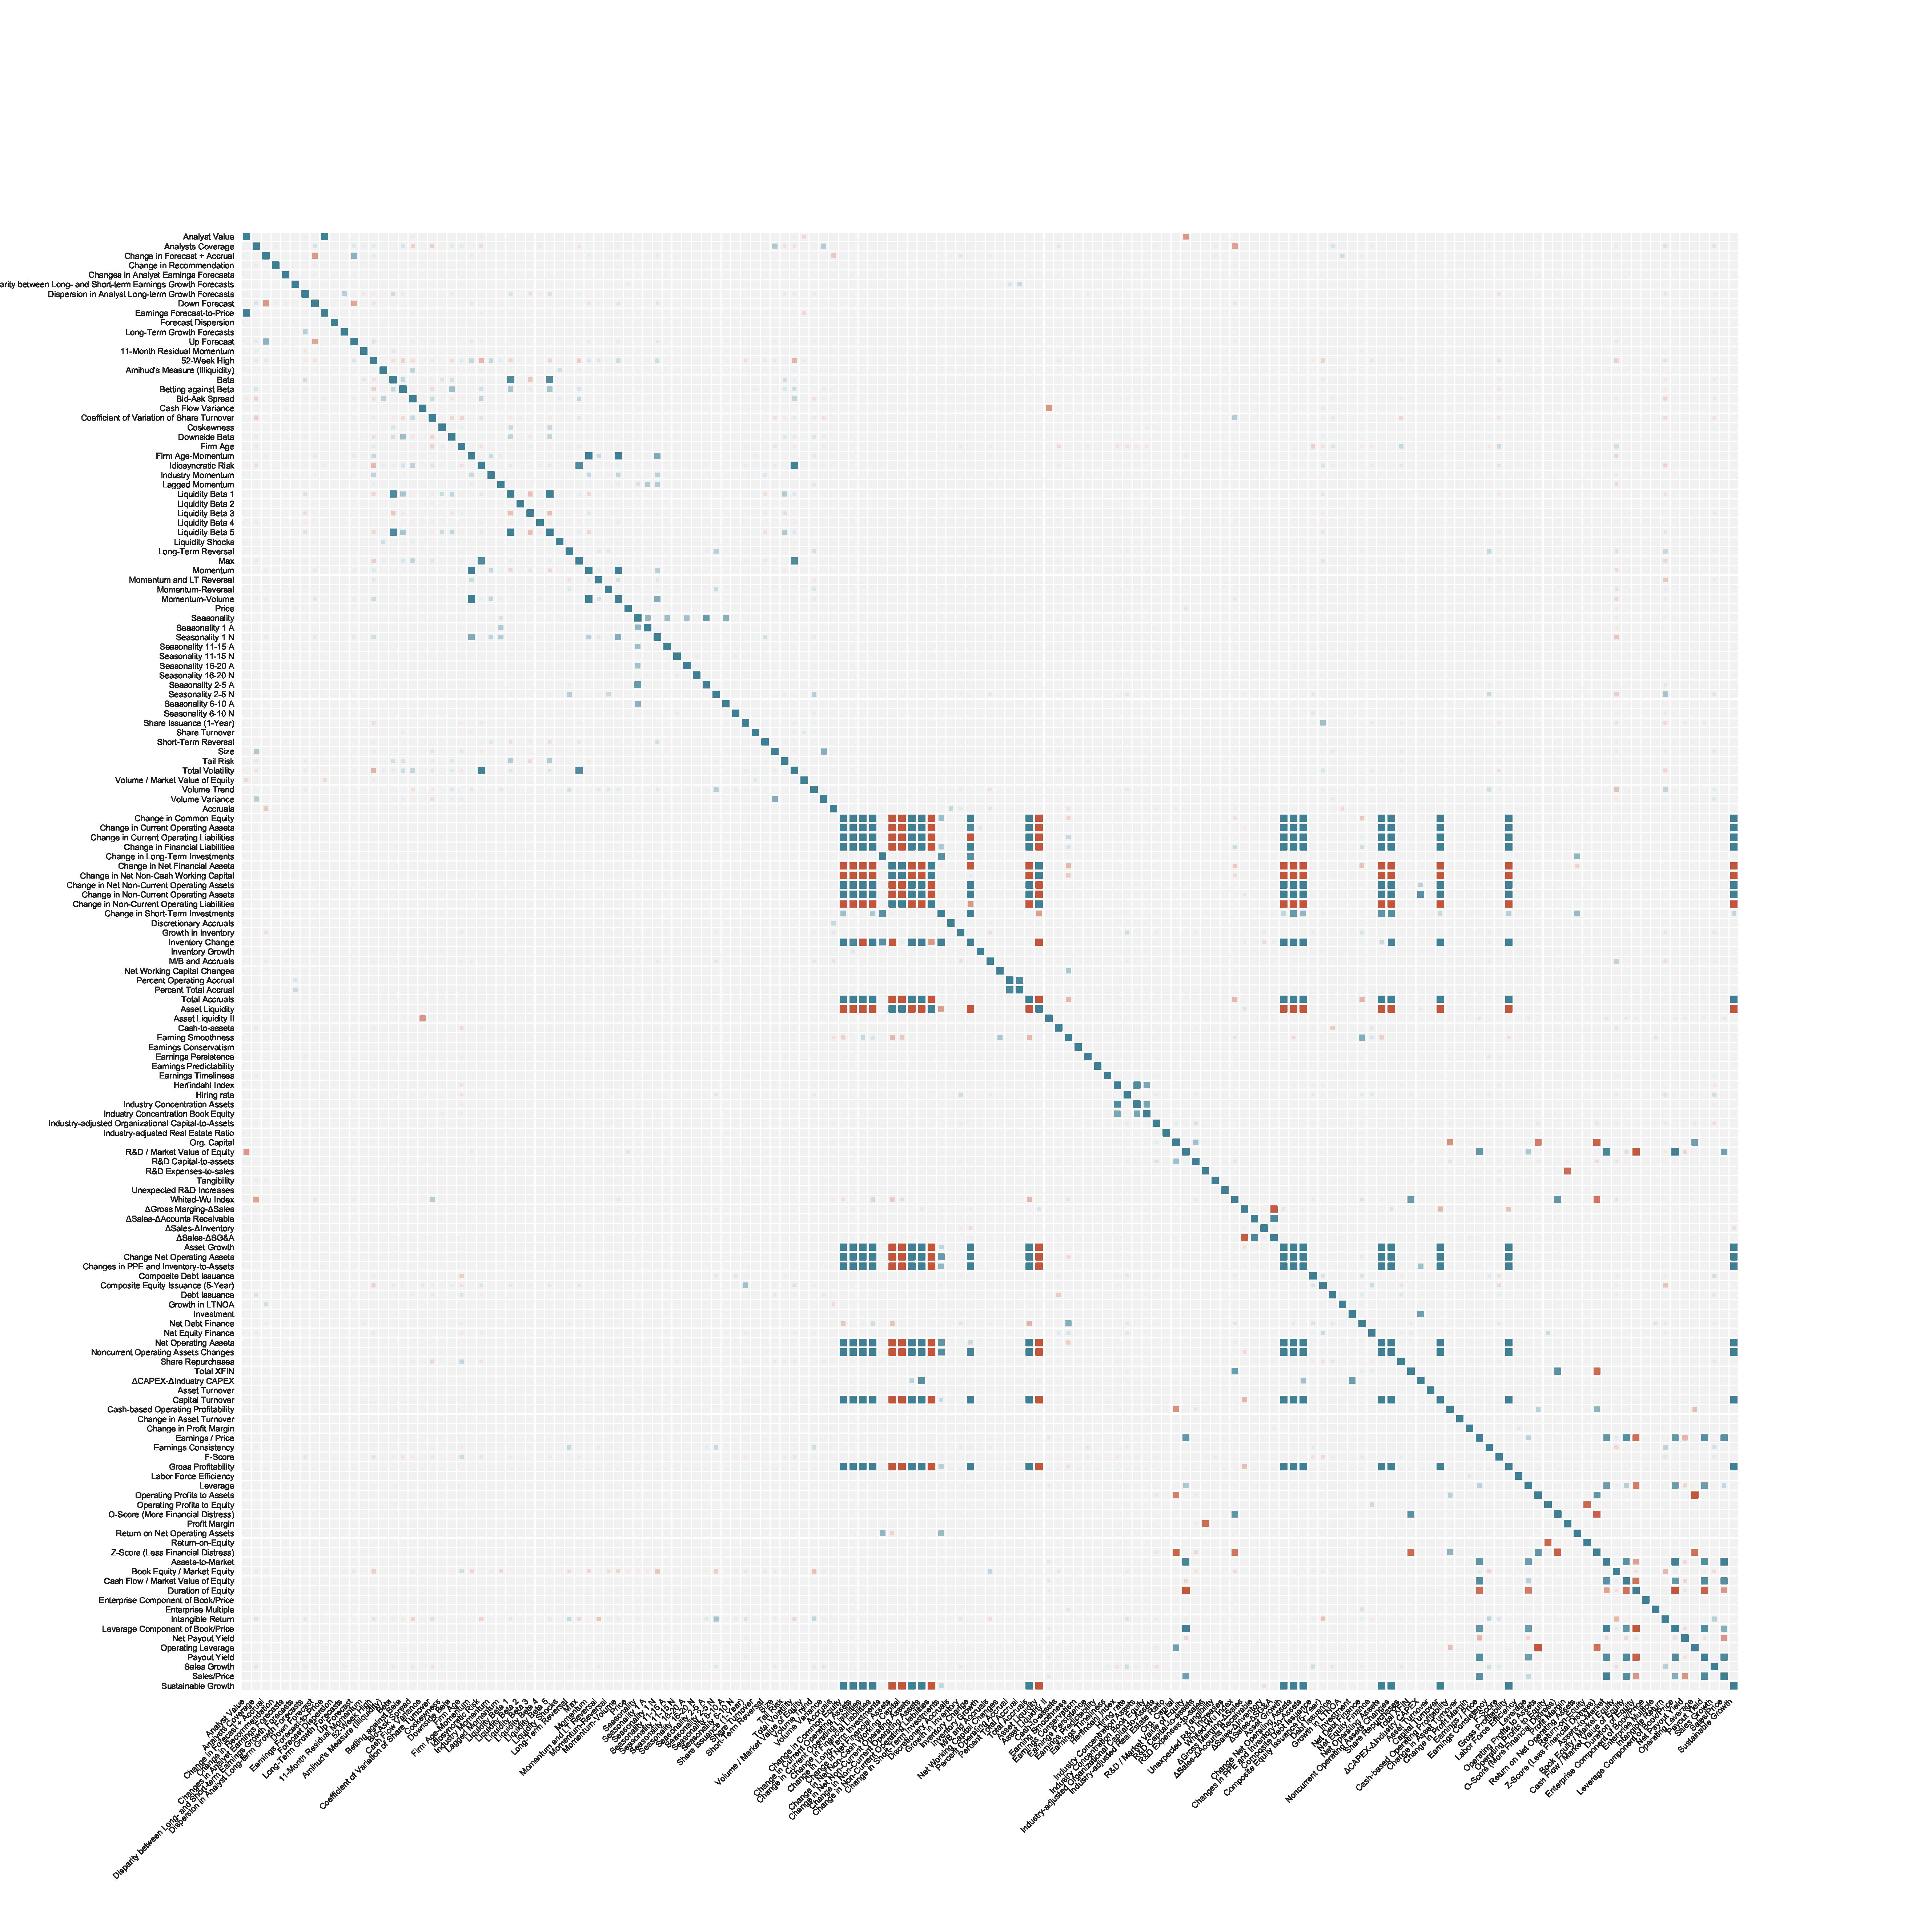
\includegraphics[width=\textwidth,height=\textheight,keepaspectratio]{Figures/corrplot.pdf}
			\caption{Correlation Matrix of the Anomalies}
			\label{fig:corrplot}
		\end{figure}
	\end{center}
	
	
	\begin{center}
		\begin{figure}
			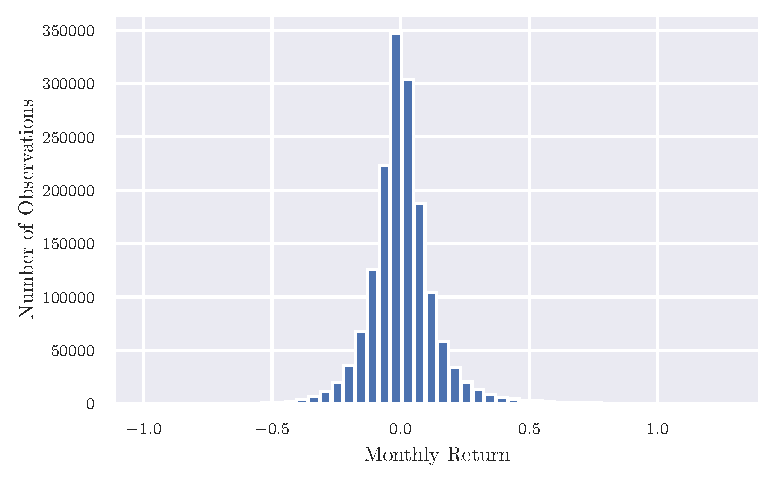
\includegraphics{Figures/hist_returns.pdf}
			\caption{Histogram of Monthly Returns}
			\label{fig:hist_returns}
		\end{figure}
	\end{center}


\section{Methodology}

	I train 5 distinct feed-forward neural networks, each with 9 different random seeds. The architecture and training follows closely \cite{gu2020empirical}, which represents very standard neural networks used in the task of equity return prediction from anomaly data. I compare the performance to that reached in the very same paper. Next, I interpret the neural networks using feature importance and investigate whether this interpretability is robust across different random seeds. I also investigate whether the interpretation of the model is stable in time. This  section describes the methodological issues related, in this order, to the model's architecture, training, performance evaluation and interpretation of the neural networks employed in this thesis.
	
	\subsection{Architecture of the Neural Networks}
	
	The prediction task is to predict stock's return in the following month using a set of the stock's charasteristics calculated as of the current month. My neural networks' architecture is a standard one for this prediction task and identical to \cite{gu2020empirical}. In summary: all networks are feed-forward with the input dimension 30 and the output dimension 1; models of 5 different depths are used, with 1, 2, 3, 4, and 5 hidden layers consisting of 32, 16, 8, 4, and 2 neurons each respectively; all layers are fully connected, with batch-normalization \citep{ioffe2015batch} and ReLU activations on all hidden layers. As this is a regression problem, there is no activation on the output layer. The weights are regularized using l1 penalty. The following explains and motivates these choices in detail, but a reader who is already well-versed in neural network design can easily skip to the next subsection, concerned with training. 
	
	First, let us describe a feed-forward neural network in general terms (e.g., \cite{goodfellow2016deep}). A feed-forward neural network can be represented as directed graph, consisting of several layers. The input layer of $N$ neurons (nodes in the graph). This layer is connected to the next layer of neurons (the first hidden layer) by edges going from each input neuron to each hidden layer neuron. When each neuron of a layer is connected to each neuron in the next layer, we say that the two layers are fully connected. Each edge connecting two neurons is parametrized by a single trainable weight. More hidden layers can be connected to the previous hidden layer in the same fashion. Finally, the last hidden layer is connected, again, fully, to the output layer, which is the final prediction.
	
	This directed graph is a representation of the computation performed by the neural network to get from the input to the output. The values of a given hidden layer, \vec{h}, are computed using the previous layer's values $\vec{x}$, and the matrix of weights on the edges $\vec{W}$ using sum of products: 
	
	\begin{equation}
		\vec{h} = f(\vec{W}\vec{x})
	\end{equation}
	
	or written element-wise, the value of neuron $h_i$ in the hidden layer is computed as 
	
	\begin{equation}
		h_i = f \left( \sum_{j}w_{i,j}x_j \right)
	\end{equation}
	
	where the function $f$ is a non-linear activation function, such as the rectified linear unit (ReLU):
	
	\[
		f(z) = \text{ReLU}(z) =   
			\begin{cases}
				1 & \text{if } z \geq 0\\
				0 & \text{otherwise}
			\end{cases}.
	\]
	
	The output layer is computed using the last hidden layer in the same manner, except in the case of regression there is no activation function. Denoting $\vec{V}$ the weights on the last edges and $\vec{h}$ the output of the last hidden layer, the output of the neural network $\vec{o}$ has the elements: 
	
	\begin{equation}
		o_i = \sum_{j}v_{i,j} h_j.
	\end{equation}
	
	In this thesis, the output is a scalar, so this further simplifies to 
	
	\begin{equation}
		o = \sum_{j}v_{j} h_j.
	\end{equation}
	
	Obviously, in the case of neural network without hidden layers, the model simplifies to linear regression. Adding a hidden layer, which is a non-linear interaction of the previous layer's neurons, the input features are allowed to interact in any manner. Essentially, a hidden layer represents the input features in a sparser manner, generating more abstract, all-encompassing information from them. This information then enters the next hidden layer and the information is made yet more high-level. This continues until the output layer, which produces the most high-level information: the prediction. In this way, the network learns to find relationships between the features such that they predict the target (here, the return) well. The network's depth corresponds to the complexity of the model: the model with a single hidden layer can be considered the least complex one, as the inputs only enter one non-linear interaction, and the complexity increases up to 5 hidden layers, where the most abstract or high-level information is extracted. 
	
	In this thesis, a neural network takes input of 30 real numbers (the stock's characteristics at given time point, dimension of the input layer) and propagates it through the series of hidden layers to produce the return prediction.	A choice must be made as to the number of hidden layers and number of neurons in each layer. While on optimal architecture can be searched for, here it is not necessary, as reaching the best possible performance is not the goal of this thesis. Instead, I follow \cite{gu2020empirical} and use the same numbers of layers and neurons: I train models of 5 different depths (1, 2, 3, 4, and 5 hidden layers), with 32 neurons in the first layer, 16 in the second layer, 8 in the third, 4 in the fourth and 2 in the fifth.  
	
	In addition, I add a batch-normalization layer \citep{ioffe2015batch} after every hidden layer, again in line with  \cite{gu2020empirical}. This changes the above formula for hidden layer values to: 
	
	\begin{equation}
		\vec{h} = \text{ReLU}(\text{BN}(\vec{W}\vec{x}))
	\end{equation}
	
	where $\text{BN}$ represents the batch-normalization operation. The operation simply normalizes its input data (subtracts sample mean and divides by sample variance). The data is split to batches to improve computing speed of the operation. The operation helps with multiple aspects of training the neural networks, as it prevents the values coming out of a hidden layer from being extreme. This helps to regularize the network and also speeds up the training. Importantly, it helps with the problem of "internal covariate shift", where the distributions of inputs to hidden layers are shifted relative to their validation and testing counterparts, which harms the predictive power and the convergence. By demeaning and standardizing the data, batch normalization preserves the information contained in the hidden layer while preventing the covariate shift \citep{ioffe2015batch}. 
	
	
	\subsection{Training, Regularization and Hyperparameter Tuning}
	
	In general terms, training any neural network amounts to searching for such weights on its edges such that the loss on the training data (typically reflecting the prediction error) is small. The optimization is done numerically, by iteratively adjusting the weights so that a loss is gradually decreasing. At the beginning of training, the model is initialized with small random weights, where the random state is determined using the so-called random seed. Prediction is computed using these weights, which are then adjusted using the negative gradient of the loss. This is applied iteratively until a stopping criterion is met and the final weights are extracted. This thesis uses mean squared error as the loss, as the prediction task is a regression.
	
	The data is fed to the network in so-called batches, meaning that several inputs are processed together and the weight update is calculated across the whole batch. When all training data-points have been fed to the network exactly once, we say one epoch has passed. This is repeated for a number of epochs. I use batch size of 5,000, which is enough for processing the data reasonably fast while not overflowing the memory. I use 100 epochs in line with \cite{gu2020empirical}, but this number is never actually reached during the training (it works just as an upper limit), due to early stopping, as explained below.
	
	There are several optimizers one can use to descend the slopes of the loss function. In line with \cite{gu2020empirical}, I use Adam optimizer. The advantage of Adam is two-fold. First, it essentially lowers the learning rate as the training progresses. The learning rate governs how much the weights are adjusted in a given direction (in the direction of negative gradient of the loss in the simple case of Stochastic Gradient Descent optimizer). Shrinking the learning rate gradually allows faster learning at the beginning of the training and a more nuanced convergence near the optimum [TODO add citation]. [TODO refresh the theory behind using Adam and describe the advantages better]. (In about 1\% of the cases, the optimized model learns to predict just the average of the training data. I retrain these models using Stochastic Gradient Descent optimizer with Nesterov momentum 0.99.)
	
	Neural networks are non-parametric way of modeling the relationship between the predictors and the predicted variables, in the sense that there is no a priori assumption made about the functional form of the relationship. In fact, the Universal Approximation Theorem shows that with already a single hidden layer, the network outlined above is able to approximate any "well-behaved" function arbitrarily well. This is directly opposed to the linear approach, where we fit the relationship between inputs and outputs assuming a linear functional form. 
	
	This necessarily means that neural networks are prone to overfitting the training data. An overfitted model performs well on the training data and poorly on previously unseen data. This is a problem, as the point of having a model in the first place is to be able to draw general conclusions and predict from new data. This is why the models are evaluated solely on held-out data (testing sample), which is disjoint from both training and validation sample, both for purposes of measuring performance and interpreting the models. In addition, there is a number of methods that can be used to prevent overfitting on the training data in the first place, commonly called regularization. The goal is to limit the training process to prevent overfitting while leaving enough room for learning. I use the same regularization techniques as \cite{gu2020empirical}, namely, learning rate shrinkage, batch normalization, early stopping, weight regularization, and ensembling. I have already discussed the use of batch normalization and learning rate shrinkage. I now describe how I use the remaining methods. 
	
	Early stopping amounts to ceasing the training at some earlier point than reaching the pre-specified number of epochs. To determine that point, one can evaluate the model's predictive power after each epoch. A subsample of the data disjoint from training data (called validation sample) is used for the evaluation. This simulates the out-of-sample performance. When the validation loss increases for $k$ consecutive epochs ($k$ is called patience), training is stopped. In line with \cite{gu2020empirical}, I use patience of 5. 
	
	Weight regularization allows to punish the model for finding too big weights, as large weights are a symptom of overfitting. The size of weights can be measured as their L2 or L1 norm, L1 norm is used here. The strength of the weight regularization is chosen as a hyperparameter on validation data and line with \cite{gu2020empirical}, as described below in the section on hyperparameter tuning.
	
	Ensembling, averaging the predictions of multiple models, is widely discussed in the Literature Review. It can be considered a regularization technique, as different models can overfit to training data differently, their average takes out this error and thus is able to generalize better. I construct the ensembles in a common way and in line with \cite{gu2020empirical}, by averaging the same model across its different random seeds. I use 9 random seeds for each model (that is, for each train-validation-test split and each architecture). As models with different random seed can be trained in parallel, this does not place a burden on the computation time.
		
	The remaining modeling choices (starting learning rate and strength of l1 regularization) are done using hyperparameter tuning. The hyperparameters discussed so far are not very data-specific, so it suffices to choose them using prior literature: I use \cite{gu2020empirical}, as we share the exact same prediction task. However, there are parameters that are very data-specific, and must therefore be chosen using the data. Choosing the parameters on the training data would lead to overfitting, which is why they are selected using a sample disjoint from training data, called validation sample. This is called hyperparameter tuning. Specifically, I tune the learning rate and the strength of l1 regularization. Each model (each of its 9 random seeds) is run 20 independent times, each time sampling the learning rate and the l1 hyperparameters randomly from pre-specified intervals using logarithmic distribution. The intervals are $\left[1\mathrm{e}{-3}, 1\mathrm{e}{-2}\right]$ and $\left[1\mathrm{e}{-5}, 1\mathrm{e}{-3}\right]$ respectively, again in line with \cite{gu2020empirical}. A single best instance is then selected, as determined by predictive performance of the model on the validation set.
	
	The train-validation-test split is done as follows. There are 29 years of data in the entire dataset, with rather evenly distributed observations from 1990 to 2018. The first 12 years of data are used as training set. The next 12 years are used as the validation set, and the year after that as the test set. To investigate how the model changes in time, more splits are performed: each year, the training data is rolled forward using expanding window (that is, taking 13 years from the beginning of the dataset, 14, 15 etc.). Validation set is rolled forward using fixed window (always consisting of 12 years) and starts directly at the end of the corresponding training set, and the test set is rolled forward also using fixed window (always consisting of 1 year) and starts directly at the end of the corresponding validation set. The train-validation-test split can be therefore summarized as 12-12-1, 13-12-1, 14-12-1, 15-12-1 and 16-12-1, where the last split uses all 29 years in the dataset. Each time a different split is taken, the model is retrained from scratch. This approach reflects that of \cite{gu2020empirical}, adjusted appropriately to my shorter dataset (29 years instead of 60) and is used instead of cross-validation so that the temporal ordering of the data is preserved (the model is trained on the past and evaluated on the future, never in the reverse).    


	\subsection{Performance Evaluation}
	The predictive performance of the models is measured using several metrics – $R^2$, root-mean-squared error (RMSE) and mean-absolute error (MAE). As all the models are evaluated on the test set, whose data were never used during training and hyperparameter tuning, we call all these metrics out-of-sample (OOS), as opposed to in-sample. It is important to use the out-of-sample metrics to be sure that the results are not due to overfitting. 
	
	$R^2$ is here defined slightly differently than usual:
	
	\begin{equation}
		R^2_{OOS} = 1 - \frac{ \sum_{(i,t)\in T_3} \left(r_{i,t+1}-	\hat{r}_{i, t+1}\right) ^2}{\sum_{(i,t)\in T_3} r_{i,t+1}^2}, 		
	\end{equation}
	
	where $T_3$ indicates the testing sample. This is also the definition of $R^2$ used by \cite{gu2020empirical}. As the usual $R^2$, it measures how much of the variance in the predicted variable (here, return) is explained by the model, but it is distinct from the usual $R^2$ in that there is no demeaning in the denominator. This means that instead of comparing the forecasts to the naive forecast of average return, the metric compares predictions to the naive forecast of zero returns. This is because in the task of predicting individual stock returns, forecasts using global average often underperfom those using just zero, so using the usual $R^2$ definition would be too low a hurdle \citep{gu2020empirical}. 
	
	The RMSE is defined in the usual manner:   
	
	\begin{equation}
		RMSE_{OOS} = \sqrt{ \frac{1}{|T_3|} \sum_{(i,t)\in T_3} \left(r_{i,t+1}-	\hat{r}_{i, t+1}\right) ^2},	
	\end{equation}
	
	and represents the average squared error of the prediction after taking a root of it, which is done so that the final measure is directly comparable in scale to the original returns. Note that it is very similar to the numerator of $R^2$.
	
	The MAE is defined as usual as well: 
	
	\begin{equation}
		MAE_{OOS} = \frac{1}{|T_3|} \sum_{(i,t)\in T_3} |r_{i,t+1}-	\hat{r}_{i, t+1}|
	\end{equation}
	
	and differs from RMSE just in taking absolute value of the error instead of square, which gives same weight to large errors as to the small ones, as opposed to RMSE where large errors have larger weights (rising with their square). 
	
	
	\subsection{Interpretation}
	
	Possibly the most straightforward way of interpreting any model is to show how individual predictors contribute to the prediction, in other words, which explanatory variables matter the most and which are less important. This notion is called \textit{global feature importance} and can be generally thought of as the ML counterpart to coefficients in a linear regression. The measure is considered to be global, since it explains how the model decides overall. This is opposed to analyzing individual predictions, which can also be done and is called local feature importance. However, to understand the model on the highest level, it is useful to study the importances in aggregate, that is, globally. This thesis employs two measures of global feature importance, Model Reliance \citep{fisher2019all} and Integrated Gradients \citep{sundararajan2017axiomatic}. The reasons behind choosing these measures as well as their theoretical underpinnings are explained in the Literature Review. This section describes the technical aspects of the measures' construction.
	
	\subsubsection{Model Reliance}
		The first measure of global feature importance used is Model Reliance \citep{fisher2019all}. It is based on the idea that if a feature is important for making prediction, then distorting the feature by adding noise to it will damage prediction performance. Vice versa, if distorting a feature leaves the prediction performance relatively intact, that feature can be considered unimportant for the prediction. Thus, denoting  the prediction function (such as an ML model) $f$, Model Reliance of  $f$ on random variable $X$ can be \textit{informally} defined as
		
		\begin{equation}
			MR(f):=\frac{\text{Expected loss of \textit{f} under noise}}{\text{Expected loss of \textit{f} without noise}},
		\end{equation}
		
		where the noise renders the random variable $X$ completely uninformative of the predicted variable while it at the same time does \textit{not} change the marginal distribution of $X$. More specifically, denote the predicted random variable as $Y$ and consider $X_1$ and $X_2$ as two explanatory random variables. The expected loss of $f$ can be then denoted as 
		
		\begin{equation}
			e_{\text{orig}}(f):= \mathbb{E} L(f,(Y,X_1, X_2)).
		\end{equation} 
		
		Further denote $X_1^s$ as random variable following the same marginal distribution as $X_1$, but independent of $Y$. 
		
		Then the expected loss of $f$ under noise, which distorts $X_1$ to $X_1^s$, can be denoted as 
		
		\begin{equation}
			e_{\text{switch}}(f):= \mathbb{E} L(f,(Y,X_1^s, X_2)).
		\end{equation} 
		
		Finally, Model Reliance can be \textit{formally} defined as 
		
		\begin{equation}
			MR(f):=\frac{e_{\text{switch}}(f)}{e_{\text{orig}}(f)}
		\end{equation}
		
		To see the intuition behind this formula, consider first the case that $X$ is very informative of $Y$. Then, 	$e_{\text{switch}}$ is much larger than $e_{\text{orig}}$ and Model Reliance is larger than 1. The more $X$ is informative of $Y$, the larger the  Model Reliance of $f$ on $X$ – the more the model \textit{relies} on the feature to make the prediction. In the case when Model Reliance is exactly 1, the feature can be considered unimportant, as completely distorting it does not change the model's loss. Model Reliance can also be less than one, in the case that the distorted feature actually perform better than the original feature.
				
		The sample estimate of $e_{\text{orig}}(f)$ is the loss used in the model's training. Denoting the target as $\vec{y} \in \mathbb{R}^N$ and consider two features $\vec{x_1}, \vec{x_2} \in \mathbb{R}^{N}$:
		
		\begin{equation}
			\hat{e}_{\text{orig}}(f):= \frac{1}{N} \sum_{i=1}^{N} L\left(f, (y_i, x_{1_i}, x_{2_i}) \right)
		\end{equation} 
		
		The sample estimate of $e_{\text{switch}}(f)$ can be done in two different ways, either by randomly permuting the values of the given feature or by dividing the feature's values in halves and the switching the halves. This thesis uses the latter, as it is computationally less demanding. (In both cases, the rest of the features and the predicted variables are intact.) It follows that the sample estimate of $e_{\text{switch}}(f)$ can be calculated as
		
		
		\begin{equation}
			\begin{split}
				\hat{e}_{\text{switch}}(f):= & \frac{1}{2 \lfloor N/2 \rfloor} \sum_{i=1}^{\lfloor N/2 \rfloor} L \left(f, \left( y_i, x_{1_{i+\lfloor N/2 \rfloor}}, x_{2_{i}} \right) \right) + \\ 
				& + L \left( f, \left(y_{i+\lfloor N/2 \rfloor}, x_{1_{i}}, x_{2_{i+\lfloor N/2 \rfloor}} \right) \right). 
			\end{split}
		\end{equation}
		
		This is simply the loss of the prediction using the same data as original, but with values in the feature $\vec{x_1}$ split in half and the halves swapped, leaving the other features (here, $\vec{x_2}$) and the predicted variable $y$ unchanged. (If $N$ is even, the split in half can be performed exactly, and if $N$ is odd, the last observation in the dataset is not used and the split is then performed in the same way as if $N$ is even.) The extension to the case with more than two features is straightforward: when calculating Model Reliance of feature $\vec{x_1}$, we disturbed the values in $\vec{x}_1$, leaving $\vec{y}$ and $\vec{x_2}$ unchanged. If we additionally have, say, $\vec{x_3}$ and $\vec{x_4}$, they are treated in the same way as $\vec{x_2}$, that is, unchanged. 
		
		Finally, the sample estimate of Model Reliance on a given feature is: 
		
		\begin{equation}
			\widehat{MR}(f):=\frac{\hat{e}_{\text{switch}}(f)}{\hat{e}_{\text{orig}}(f)}.
		\end{equation}
			
		That is, when calculating reliance of the model on a given feature, two predictions are made using the model: one is the usual one, with all features as well as the target undisturbed, the other is almost the same, except that we have disturbed the given feature (and the given feature only) by swapping halves of its values. The loss of both predictions is then computed as usual. Model Reliance is then the ratio of these two losses, the disturbed loss divided by the undisturbed one.   
		
		
	
		
	\subsubsection{Integrated Gradients}
		Another measure of feature importance is Integrated Gradients \citep{sundararajan2017axiomatic}. It considers the gradient of the prediction with respect to the predictors. If a small change in a predictor's value has large effect on the prediction, the value of the gradient is large. The measure is computed locally, i.e., for each observation separately, as follows:
		
		Again, denote $f: \mathbb{R}^k \rightarrow \mathbb{R}$ the prediction function (here, the NN model). Further, denote $\vec{z} \in  \mathbb{R}^k$ a single input with $k$ scalar elements, where $k$ denotes the total number of features (here, 30). Let $\vec{z'} \in  \mathbb{R}^k$ be a \textit{baseline input}, an observation that can be considered as a point from which the other observations depart. (For example, in case of inputs being images, the baseline can be a black image. In this thesis, it is a vector of zeros, as motivated below.) 
		
		For simplicity of the notation, assume that $f: \mathbb{R}^k \rightarrow [0,1]$. The Integrated Gradient of $i^{th}$ feature of the input $\vec{z}$ is defined as 
		
		\begin{equation}
			IG_i(\vec{z}) := (z_i - z_i') \int_{\alpha=0}^{1} \frac{\partial f(\vec{z'} + \alpha(\vec{z}-\vec{z'}))}{\partial z_i}d\alpha,
		\end{equation}
		
		where $\frac{\partial f(\vec{z})}{\partial z_i}$ stands for the gradient of $f(\vec{z})$ along the $i^{th}$ dimension. This means that the measure considers a straight path in $\mathbb{R}^k$ from the baseline input ${\vec{z}'}$ to the given input ${\vec{z}}$ and calculates the gradient of prediction at all points along that path. The Integrated Gradient measure cumulates these gradients by taking the integral across the path.  
		
		To calculate the Integrated Gradient of $i^{th}$ feature of the input $\vec{z}$ empirically, it is necessary to approximate the integral by summation across several points along the straightline path  \citep{sundararajan2017axiomatic}. That is:  
		
		\begin{equation}
			IG_i^{\text{approx}}(\vec{z}) := (z_i - z_i') \sum_{k=1}^{m} \frac{\partial f(\vec{z'} + \frac{k}{m}(\vec{z}-\vec{z'}))}{\partial z_i}\frac{1}{m},
		\end{equation} 

		where $m$, called the \textit{step size}, is the number of the steps in the Reimman approximation of the integral, here, the number of points along the straightline path at which evaluate the gradient. 
		
		Two implementation decisions must be made when calculating the Integrated Gradients: first, choosing the right baseline input, and second, choosing the right the step size. First, the baseline input should be chosen such that it can be interpreted as "no signal". Additionally, the authors recommend to check that the model's prediction at baseline is around zero. This is important because it allows to use Integrated Gradient to explain the prediction as a function of the input, and not as of the input and the baseline. In this thesis, there are two possible baselines: random noise and all-zero input. The latter was chosen, as it is natural to interpret as "no signal": all the features are normalized between -1 and 1 and have a mean of 0, thus, an all-zero input can be considered a natural point of departure. The predictions for the all-zero input are around zero, as required [TODO verify]. Second, the step size should be chosen such that the approximation is good enough: the authors recommend to check that the attributions approximately sum up to the difference between the prediction at $\vec{z}$ and at $\vec{z'}$. Given that the latter is around zero, it remains to check that the attributions for $\vec{z}$ sum up to the prediction at $\vec{z}$. (Note that this is a verification of passing the Completness Axiom, see Literature Review.) This thesis uses the step size of 50, which passes this summation check comfortably [TODO verify].  
	\chapter{Results}
\label{chap:res}

\section{Performance Evaluation}
	
	\subsection{Predictive Ability}
		\label{chap:predictive_ability}
	
		Table \ref{tab:performance} shows the predictive ability of the networks. All four nets (NN1 to NN4) are rather similar in the mean errors of their predictions. The Mean Absolute Error is around 0.075, which is a rather high portion of the variability in monthly return (mean monthly return is 0.005 with 0.051 standard deviation).  However, these relatively high prediction errors are a commonplace in stock returns prediction and are due to the low signal-to noise ratio of financial data in general. The $R^2$ shows the fraction of variability in data explained by the model, above that of the naive forecast of zero return. The values range from 0.022\% for NN4 across 0.039\% for NN3 to 0.21\% for NN1 and finally 0.25\% for NN2. These numbers are somewhat lower than in \cite{gu2020empirical}, who report $R^2$ of around 0.35\%, but discussion with the authors of \cite{tobek2020does} reveals that the $R^2$ values found in this thesis are actually commonplace in the stock returns prediction task [TODO I can't find a proper citation, nobody seems to report R2].    
		
		Figure \ref{fig:r2} shows a decomposition of $R^2$ into deciles by return: the stocks are grouped into 10 groups, corresponding to the decile of their return, and $R^2$ is calculated separately for each decile. The results show that the predictive ability of the networks is higher the higher the return: put simply, the networks are good at predicting returns of stocks that end up performing very well and bad at predicting mediocre returns. In the top 10\% of stocks (decile 100), the networks explain as much as  0.5\% to 1\% of returns variability above naive forecast of 0. The performance is similarly good in the 80th and the 90th decile, but seems to be decreasing. For the 60th, 50th, 40th decile, the performance ranges around 0, meaning that the models explain as much variance as the naive forecast of 0 around the center of the returns distribution. For 30th decile, all models actually under-perform the naive 0 forecast (negative values of $R^2$). Some models (NN1 and NN3) seem to improve in the lowest decile, (barely) climbing out of the negative $R^2$ territory. This generally indicates that the models may be better at predicting returns of winners than mediocre and poorly-performing stocks, at least in terms of the explained variance of the data.    
		
		\begin{figure}	
			\centering		
			\begin{subfigure}[t]{\textwidth}
				\centering	
				\begin{tabular}{lrrrrrr}
\toprule
{} &     LR &    NN1 &    NN2 &    NN3 &    NN4 &    NN5 \\
\midrule
R Square                &   0.09 &   0.30 &  -0.32 &  -1.22 &   0.21 &   0.48 \\
Mean Squared Error      &   1.88 &   2.10 &   2.20 &   2.22 &   2.12 &   2.38 \\
Mean Absolute Error     &   7.86 &   7.85 &   7.90 &   7.94 &   7.76 &   7.82 \\
Root Mean Squared Error &  13.63 &  13.62 &  13.66 &  13.71 &  13.67 &  13.61 \\
\bottomrule
\end{tabular}

				\caption{All Out-of-Sample Measures of Predictive Ability}
				\label{tab:performance}
			\end{subfigure}
			
			\begin{subfigure}[t]{\textwidth}
				\includegraphics[width=\textwidth,height=\textheight,keepaspectratio]{Figures/r2.pdf}
				\caption{Decomposition of Out-of-Sample $R^2$ into Deciles}
				\label{fig:r2}
			\end{subfigure}
			\caption{Out-of-Sample Predictive Ability of the Networks}
			\medskip
			\small
			NN1 to NN4 stand for neural networks of respective depths. Panel (\subref{tab:performance}) shows predictive ability of all models. All metrics are calculated out-of-sample and are defined in Section \ref{chap:model_evaluation}. $R^2$ is in percentage points. Panel (\subref{fig:r2}) decomposes the last row in Panel (\subref{tab:performance}), $R^2$, into deciles. Specifically, out-of-sample predictions of each network are split into 10 subsets based on decile of the actual return. $R^2$ of the prediction is then calculated on the individual subsets. For example, decile 10 (100) denotes the bottom (top) 10\% of observations by return (all deciles are mutually exclusive by construction). The figure shows that all networks are able to predict high returns well (decile 80, 90 and 100), but they under-perform the naive prediction of 0 (negative $R^2$) in the low to medium return deciles (30 to 60). 
			\label{fig:predictive_ability}
		\end{figure}     
		

	\subsection{Profitability of Trading Strategy (Backtest)}
		\label{chap:backtest}
		
		\begin{figure}	
			\centering		
			\begin{subfigure}[t]{\textwidth}
				\centering	
				\includegraphics[width=\textwidth,height=\textheight,keepaspectratio]{Figures/backtest_cumreturns_models.pdf}
				\caption{Cumulative Returns on the Long-Short Portfolios}
				\label{fig:backtest_cumreturns_models}
			\end{subfigure}
			
			\begin{subfigure}[t]{\textwidth}
				\includegraphics[width=\textwidth,height=\textheight,keepaspectratio]{Figures/backtest_cumreturns_ls.pdf}
				\caption{Long and Short Legs of the Portfolio (NN1)}
				\label{fig:backtest_cumreturns_ls}
			\end{subfigure}
			\caption{Cumulative Returns on the Long-Short Portfolio}
			\medskip
			\small
			[TODO change labels in Panel b: Remove word Gross from ylabel, change label All Stocks to Market in legend]. NN1 to NN4 stand for neural networks of respective depths. As described in \ref{chap:met_backtest}, the portfolios are constructed by letting each network make out-of-sample prediction of returns in the next month, ordering the stocks by predicted return from highest to lowest, buying the top 10\% of stocks and short-selling the bottom 10\%. The Market portfolio is constructed by buying the entire universe of stocks available in the given month. All portfolios are equal-weighted. Panel (\subref{fig:backtest_cumreturns_models}) shows the long-short portfolios of all models, while Panel (\subref{fig:backtest_cumreturns_ls}) decomposes the long-short return of NN1 into the long and short legs. 
			\label{fig:cumulative_return}
		\end{figure}     
		
		
		\begin{figure}	
			\centering		
			\begin{subfigure}[t]{\textwidth}
				\centering	
				\begin{tabular}{lrrrrr}
\toprule
{} &  Market &    NN1 &    NN2 &    NN3 &    NN4 \\
\midrule
Mean               &   0.005 &  0.014 &  0.012 &  0.009 &  0.014 \\
Mean (Yearly)      &   0.072 &  0.191 &  0.153 &  0.122 &  0.183 \\
Standard Deviation &   0.051 &  0.043 &  0.039 &  0.042 &  0.040 \\
Sharpe Ratio       &   0.325 &  1.160 &  1.047 &  0.712 &  1.229 \\
Skewness           &  -0.633 & -0.148 & -0.133 &  0.571 &  0.574 \\
Kurtosis           &   2.118 &  2.640 &  2.504 &  2.850 &  3.020 \\
Max Drawdown       &  -0.584 & -0.225 & -0.324 & -0.272 & -0.172 \\
\bottomrule
\end{tabular}

				\caption{Descriptive Statistics of Returns on Long-Short Portfolios}
				\label{tab:backtest_descriptives_models}
			\end{subfigure}
			
			\begin{subfigure}[t]{\textwidth}
				\includegraphics[width=\textwidth,height=\textheight,keepaspectratio]{Figures/backtest_histogram.pdf}
				\caption{Histogram of Monthly Returns on the Long-Short Portfolio Generated by NN1}
				\label{fig:backtest_histogram}
			\end{subfigure}
			\caption{Descriptive Statistics of the Returns on the Long-Short Portfolios}
			\medskip
			\small
			As described in \ref{chap:met_backtest}, the portfolios are constructed by letting each network make out-of-sample prediction of returns in the next month, ordering the stocks by predicted return from highest to lowest, buying the top 10\% of stocks and short-selling the bottom 10\%. The Market portfolio is constructed by buying the entire universe of stocks available in the given month. All portfolios are equal-weighted. Panel (\subref{tab:backtest_descriptives_models}) describes the distribution of the returns earn on the long-short portfolios based on the networks' out-of-sample predictions. Panel (\subref{fig:backtest_histogram}) visualizes the same information in a histogram, focusing on NN1 and Market return. 
			\label{fig:backtest_descriptives}
		\end{figure} 
			
		Table \ref{tab:backtest_descriptives_models} Figure \ref{fig:backtest_histogram}  and describe the distribution of monthly returns earned on long-short portfolios generated by the individual networks. As described in \ref{chap:met_backtest}, the portfolios are constructed by letting a network make out-of-sample prediction of returns in the next month, ordering the stocks by predicted return from highest to lowest, buying the top 10\% of stocks and short-selling the bottom 10\%. The figures also show the market return, which serves as a benchmark. All three figures show that all the networks beat the market returns by a large margin, which gives a clear sign of their ability to identify winners and losers ex ante, resulting in a profitable long-short trading strategy. The two figures are now discussed in turn in more detail.
		
		Table \ref{tab:backtest_descriptives_models} shows the descriptive statistics of monthly returns on the long-short portfolio. While the market earns 0.5\% in an average months, the networks earn more than double: 0.9\% for the worst-performing net (NN3) and 1.4\% for the best networks (NN1 and NN4). This translates to yearly return of 12, 15, 18 and 19\% (in NN3, NN2, NN4 and NN1 respectively), which comfortably beats the 7\% earned by the market. While beating the market in average return, the networks exhibit \textit{less} return volatility at the same time: the standard deviation of the market return is 0.05, while the networks' is around 0.04. This favorable risk-return trade-off is summarized in Sharpe Ratio of around 1 (compared to market's 0.3). This gives very similar performance to the prior literature: compare the Sharpe Ratios to \cite{gu2020empirical} (in brackets): 1.16 (1.16) for NN1, 1.05 (1.15) for NN2 and  1.23 (1.35) for NN4. The only exception is NN3, which has a considerably poorer Sharpe Ratio of 0.7 (1.20). \cite{tobek2020does} report Sharpe Ratios of the networks from 0.88 to 1.58, which further confirms that the performance of the networks in this thesis is state-of-the-art. The remaining rows in Table \ref{tab:backtest_descriptives_models} summarize the skewness and kurtosis of the distributions of monthly returns: NN1 and NN3 are skewed to the right, NN3 and NN4 to the left, and the tails are generally only somewhat lighter than that of standard normal distribution for all models (kurtosis from 2.5 to 3.0). Maximum Drawdown shows the loss a trader would suffer if she started trading in 2000 and existed in the least favorable moment possible: again, the networks beat the market (-0.27 to -0.32 compared to markets' -0.58), and are close to state-of-the-art (-0.15 to -0.26 in \cite{gu2020empirical} and -0.19 to -0.38 in \cite{tobek2020does}.)   
		
		Figure \ref{fig:backtest_histogram} visual illustrate the more favorable mean, standard deviation, skewness and kurtosis of the networks' return distributions than that of market's: the mean (and also all the deciles) are more to the right, the left tail is less pronounced and the right tail is also more favorable (meaning that investors experience less terrible months and more great months than when investing to the market). The somewhat lower standard deviation is also visible in the figure. Most months see a return of 0 to 2.5\%.       
		
		Figure \ref{fig:backtest_cumreturns_models} shows the returns on the very same portfolios from a time-series perspective: it shows cumulative return earned at any time point since 2000 (beginning of the out-of-sample data). Again, market return is plotted as a benchmark. All networks consistently outperform the market (again, with a slight exception of the rather poorly performing NN3 in the early years). If trading from 2000 and exiting in 2018, an investor would pocket around 400\% of the initial investment (200\% from the poorly performing NN3 and 120\% for the market). The recessions are also visible: 2003, 2008 and 2018 saw negative returns, showing as decreasing cumulative return in the figure.      
		 
		Figure \ref{fig:backtest_cumreturns_ls} shows the decomposition of the cumulative return on the long-short portfolio\footnote{The portfolio is generated by NN1. Other architectures give similar results.} to its long and short legs. The figure also shows the market return, which serves as a benchmark. IT shows that the short-sold stocks are consistently below the market and in negative numbers, which translates to profits for the short position, while the long position is at par or better than the market. The short and long position combined result in a consistent out-performance. Also note that the short position helps to protect the portfolio in the recessions: The network was able to predict the losers if 2002 and 2008 recessions, which meant that the return of the long-short portfolio was partially insulated from the economic downturn.     
		
		
		All the backtesting performance described to this point assumes that the long (short) position is created as top (bottom) 10\%  of the stocks, as ordered by predicted return. Table \ref{tab:backtest_descriptives_ls} describes how the results change if the focus of the positions would be more or less narrow (resulting in lower or higher number of firms in both positions: 8, 17, 88, 177, 177, and 355 from right to left).\footnote{The portfolio is generated by NN1. Other architectures give similar results.} The results reviewed until now are in the column 10--10 (meaning 10\% of the market is bought and 10\% short-sold). The column 20--20 represents the situation if the positions would be distributed into more firms (broader portfolios) and the columns 5--5 1--1 and 0.5--0.5 represent progressively narrower positions (less firms bought and sold). As is expected, the mean returns are higher for the narrower portfolios (as much as 44\% yearly for 1--1), but this comes at the cost of higher standard deviation (more volatile returns) and worse Maximum Drawdown. It appears that the optimum risk-return trade-off is with 5--5, which gives the highest Sharpe Ratio of 1.2. While all variants still beat the market in mean return, only 10--10 and 20--20 are less volatile than the market, which is because there are too little firms in the smaller portfolios  to ensure a decrease in volatility (e.g., 17 firms in the long and 17 in the short position for the 1--1).
		
		\begin{table}
			\centering
			\begin{tabular}{lrrrrrr}
\toprule
{} &  Market &  0.5-0.5 &    1-1 &    5-5 &  10-10 &  20-20 \\
\midrule
Mean               &   0.005 &    0.025 &  0.028 &  0.019 &  0.014 &  0.011 \\
Mean (Yearly)      &   0.072 &    0.408 &  0.440 &  0.262 &  0.191 &  0.145 \\
Standard Deviation &   0.051 &    0.111 &  0.082 &  0.053 &  0.043 &  0.033 \\
Sharpe Ratio       &   0.325 &    0.773 &  1.196 &  1.226 &  1.160 &  1.171 \\
Skewness           &  -0.633 &   -0.085 & -0.144 & -0.192 & -0.148 & -0.215 \\
Kurtosis           &   2.118 &    0.262 &  0.982 &  2.273 &  2.640 &  4.265 \\
Max Drawdown       &  -0.584 &   -0.826 & -0.567 & -0.263 & -0.225 & -0.181 \\
\bottomrule
\end{tabular}

			\caption{Descriptive Statistics of Returns on Long-Short Portfolios Generated by NN1 in Different Capital Allocations}
			\label{tab:backtest_descriptives_ls}
			\medskip 
			\small 
			As described in \ref{chap:met_backtest}, the NN1 portfolio is constructed by letting a network make out-of-sample prediction of returns in the next month, ordering the stocks by predicted return from highest to lowest, buying the top $m$\% of stocks and short-selling the bottom $n$\%. Here, $m=n$ and takes values 0.5, 1, 5, 10 and 20, which gives respectively 8, 17, 88, 177, 177, and 355 firms in the long postiion and the same number of firms in the short position. All portfolios are equal-weighted. 
		\end{table}

\section {Local Feature Importance}

	This section illustrates how individual predictions of the networks can be interpreted. Particularly, any single prediction can be decomposed in an additive manner into the effects of individual features. The measure used for this decomposition is called Integrated Gradient; its use its motivated in Section \ref{chap:local_measures} and the methodological details are discussed in Section \ref{chap:integrated_gradient}. Panel (\subref{fig:local_ig_1}) of Figure \ref{fig:local_ig} shows the values of Integrated Gradient for a single prediction. The predicted return is the sum of the values of Integrated Gradient across features. In other words, the Integrated Gradient of a single feature is exactly the change in the prediction (return) that is due to (or attributed to) that feature. Panel (\subref{fig:local_ig_100}) of the figure shows the same, but for 100 predictions. Since it is computationally demanding to plot all observations into the chart, only 100 random predictions are plotted and the figure thus serves only an illustrative purpose. To obtain a global picture from the local one, I take the mean of the absolute values. All the remaining results concerning Integrated Gradient focus on the mean across all out-of-sample predictions: if the average of absolute values is high, the features can be considered important (globally) for the predictions. [TODO I could summarize distributions as well, and not look only at the mean.]

	\begin{figure}	
		\centering		
		\begin{subfigure}[t]{\textwidth}
			\includegraphics[width=\textwidth]{Figures/local_ig_1.pdf}
			\caption{Single Prediction}
			\label{fig:local_ig_1}
		\end{subfigure}
		
		\begin{subfigure}[t]{\textwidth}
			\centering
			\includegraphics[width=\textwidth]{Figures/local_ig_100.pdf}
			\caption{100 Predictions}
			\label{fig:local_ig_100}
		\end{subfigure}
		\caption{Example of Attributing the Prediction to Individual Features using Integrated Gradient}
		\medskip
		\small
		Panel (\subref{fig:local_ig_1}) shows all values of Integrated Gradient for a single (randomly chosen) out-of-sample prediction. The prediction (return of a given stock in given month) can be attributed into individual features using Integrated Gradient. The predicted return is the sum of the shown Integrated Gradient values. Panel (\subref{fig:local_ig_100}) shows the same, but for 100 predictions. The results are calculated using the network NN1.
		\label{fig:local_ig}
	\end{figure}	

	
\section{Global Feature Importance}
	\label{chap:global_feature_importance}
	
	Figures \ref{fig:ig_ensemble} and \ref{fig:pr_ensemble} shows the values of feature importance for all features, as measured respectively by Global Integrated Gradients and Portfolio Reliance. First two sections now discuss the results for the two measures in turn, the third subsection compares the results of the two measures, and the following subsections discuss stability of the results in time and across random seeds. 
	
	\subsection{Integrated Gradient}
	
		\begin{figure}	
			\centering		
			\begin{subfigure}[t]{\textwidth}
				\includegraphics[width=\textwidth]{Figures/ig_blues.pdf}
				\caption{Values of Global Integrated Gradient}
				\label{fig:ig_blues}
			\end{subfigure}
			
			\begin{subfigure}[t]{\textwidth}
				\includegraphics[width=\textwidth]{Figures/ig_order.pdf}
				\caption{Order of Features by Importance}
				\label{fig:ig_order}
			\end{subfigure}
			\caption{Feature Importance Measured with Global Integrated Gradient}
			\medskip
			\small
			Column LR shows linear regression and columns NN1 to NN4 the neural networks of respective depths. Column Mean gives the average value across the neural networks. Panel (\subref{fig:ig_blues}) shows values of the Global Integrated Gradient for all features, for all models and shows an average share of predicted return attributed to the feature (in same scale as the return itself, i.e., percentage points).  Numerical values for Panel (\subref{fig:ig_blues}) are given in the Appendix \ref{chap:numerical_results} in Figure \ref{tab:ig_blues}. Panel (\subref{fig:ig_order}) shows ordering of features by their importance, with bright colors corresponding to high order. Label 1 --- bright yellow (30 --- black) corresponds to most (least) important feature in given model, as measured by highest (lowest) Global Integrated Gradient. 
			\label{fig:ig_ensemble}
		\end{figure}
	
		Figure \ref{fig:ig_ensemble} shows importance of all features, for all models as measured by Integrated Gradients.  In both panels, the most (least) important features appear on top (bottom) of the figure. The measure shows how much the output changes on average with a small change in values of a feature. Intuitively, if the output changes a lot with a small change in given feature, the value of Global Integrated Gradient is high and the feature is considered important for the prediction. Panel (\subref{fig:ig_blues}) shows the values of the measure, while Panel (\subref{fig:ig_order}) shows the order of the features from 1 to 30 (1 for most important).
		
		Panel (\subref{fig:ig_blues}) shows the values of the Integrated Gradient for all features (the exact numerical values are given in Appendix \ref{chap:numerical_results}). The values show how a marginal change in values of a feature influences the output of the model (the predicted return) on average. \textit{Whited-Wu Index}, the most important feature, on average changes the predicted return by around 0.3 percentage points. The same holds for \textit{52-Week High} and \textit{Earnings Forecast-to-Price}, the second and third most important features. The value 0.3 is quite high, considering that the standard deviation of return is 11.2 percentage points. The next 5 features in importance are \textit{Liquidity Beta 5}, \textit{Seasonality 6-10 A}, \textit{Short-Term Reversal}, \textit{Duration of Equity} and \textit{Liquidity Beta 3}, which on average change the predicted return by 0.2--0.1 percentage points. Next 14 features (\textit{Maximum Return} to \textit{Profit Margin}) change the prediction n by 0.1--0.05 percentage points on average, and the remaining 8 change it by less than 0.05 percentage points.
		
		In light of economic motivation behind the features (Table \ref{tab:characteristics_motivation}), the most important categories seem to be financial constraints (\textit{Whited-Wu Index}), limited attention and behavioral biases of investors (\textit{Earnings Forecast-to-Price}, \textit{52-Week High and Short-Term Reversal}), risk of illiquidity (\textit{Liquidity Beta 3 and Liquidity Beta 5}), seasonality (\textit{Seasonality 6-10 A}), and value effect (\textit{Duration of Equity}). 
		
		The figure also shows that all neural networks agree on the importance to a great extent, both in values of the measure and in the implied order of the features. This is visible in both panels as same color across a row. Additionally, the figure shows that linear regression (column LR) does not agree with the neural networks on the importance of some features, most notably, \textit{Whited-Wu Index}, \textit{Liquidity Beta 5} and \textit{Short-Term Reversal} are considered important by the networks, but very marginal by the linear regression. This is most likely because the impact of the features is not linear: either, their relationship with returns is not well-fitted by linear function, or they only impact the return through an interaction with other features. (Both the non-linearities and interaction terms are captured by the hidden layers of the networks but not by the linear regression due to the architecture of the respective models.)  	
	

	
	\subsection{Portfolio Reliance}
	
		\begin{figure}	
			\centering		
			\begin{subfigure}[t]{\textwidth}
				\includegraphics[width=\textwidth]{Figures/pr_blues.pdf}
				\caption{Values of Portfolio Reliance}
				\label{fig:pr_blues}
			\end{subfigure}
			
			\begin{subfigure}[t]{\textwidth}
				\centering
				\includegraphics[width=\textwidth]{Figures/pr_order.pdf}
				\caption{Order of Features by Importance}
				\label{fig:pr_order}
			\end{subfigure}
			\caption{Feature Importance Measured with Portfolio Reliance.}
			\medskip
			\small
			Column LR shows linear regression and columns NN1 to NN4 the neural networks of respective depths. Column Mean gives the average value across the neural networks. Panel (\subref{fig:pr_blues}) shows values of the Portfolio Reliance for all features, for all models.  Panel (\subref{fig:pr_order}) shows ordering of features by their importance, with bright colors corresponding to high order. Label 1 --- bright yellow (30 --- black) corresponds to most (least) important feature in given model, as measured by highest (lowest) Portfolio Reliance. 
			\label{fig:pr_ensemble}
		\end{figure}
		
		Figure \ref{fig:pr_ensemble} shows importance of all features, for all models as measured by Portfolio Reliance. The measure shows how important a feature is for construction of the long-short portfolios (see \ref{chap:backtest}). Specifically, values represent the decrease in return on the long-short portfolio resulting from corrupting the feature (rendering it completely uninformative by permutation of its values; the methodology behind is discussed in Chapter \ref{chap:met)). Intuitively, if the mean return on the long-short portfolio decreases a lot when the feature is corrupted, the value of Portfolio Reliance is high and the feature is considered important. Same as with Figure \ref{fig:ig_ensemble}, the most (least) important features appear on top (bottom) of the figure. Again, Panel (\subref{fig:pr_blues}) shows the values of the measure, while Panel (\subref{fig:pr_order}) shows the order of the features from 1 to 30 (1 for most important). 
			
		Panel (\subref{fig:pr_blues}) shows the values of Portfolio Reliance for all features (the exact numerical values are given in Appendix \ref{chap:numerical_results}). \textit{Whited-Wu Index} is again the most important feature. Its Portfolio Reliance value (mean across the networks) is 0.23, which means that the mean return on long-short portfolio decreases by 0.23 percentage points when \textit{Whited-Wu Index} is corrupted. Considering that the mean monthly return is around 1 percentge point (1.4 for NN1, 0.9 for NN3, other in between), it means distorting the feature takes away almost quarter of the performance. Two other features follow closely: \textit{ Earnings Forecast-to-Price} (0.215) and \textit{Volume to Market Value of Equity} (0.199). Next are four features with values between 0.138 and 0.1: \textit{52-Week High}, \textit{Seasonality 6-10 A}, \textit{Idiosyncratic Risk} and \textit{Short-Term Reversal}. Six other features have Portfolio Reliance above 0.05: \textit{Coefficient of Variation of Share Turnover}, \textit{Momentum-Reversal}, \textit{RD to Market Equity} and three seasonality measures. The rest of the variables have values close to 0 (or even slightly negative), which means they are unimportant or slighlty detrimental to the performance of the portfolios. 
		
		In terms of the economic motivation of the features\ref{tab:characteristics_motivation}, the most important groups appear to be financial constraints (Whited-Wu Index), limited attention and behavioral biases of investors (\textit{Earnings Forecast-to-Price}, \textit{52-Week High}, \textit{Short-Term Reversal}, their attitude to risk (\textit{Idiosyncratic Risk}) and illiquidity (\textit{Volume to Market Value of Equity}).  
		
		Again, the networks quite agree on the importance of individual features (albeit to a somewhat lesser extent than in Integrated Gradients, \ref{fig:ig_ensemble}). Same as with Integrated Gradients, linear regression (column LR) disagrees on the importance of \textit{Whited-Wu Index} and \textit{Short-Term Reversal}, and additionally, \textit{52-Week-High}. Again, the reasons for this are likely the same as discussed with the Integrated Gradient: these features likely have non-linear or interaction-intensive effect that the linear regression fails to capture.    
		
	\subsection{Comparison of Feature Importance Measures} 	

	Figure \ref{fig:ig_pr_comparison} compares the results of the previous two subsections, namely, feature importance as measured by Integrated Gradient and by Portfolio Reliance. There is a crucial semantical difference between the two measures. The former captures the importane of the features across the entire universe of stocks, while the latter focuses only on the long-short portfolios constructed using the networks, i.e., on prediction of the very high and very low returns. Both approaches have a merit: the former closer to the academician's interest in explaining the cross-section of stock returns, the latter answers the practicioner's question of which features the networks rely on to predict winners and loosers correctly and thus outperform the market. As shown in \ref{chap:predictive_ability}, the networks are not particularly good at explaining the entire cross-section of returns (negative $R^2$ in the medium deciles), so Portfolio Reliance may be more insightful than Integrated Gradients in terms of answering the question of what contributes to the neural networks outstanding performance.

	The figure shows that the two measures seem to agree on important features to a large extent. This is quite reassuring, since the measures are constructed completely differently, and yet their results support each other. \textit{Whited-Wu Index}, \textit{52-Week High}, \textit{Earnings Forecast-to-Price}, \textit{Seasonality 6-10 A}, and \textit{Short-Term Reversal} are among the most important features for both measures. 
	
	However, there are two features that are quite important in Integrated Gradients and unimportant in Portfolio Reliance: \textit{Liquidity Beta 5} and \textit{Lagged Momentum}. Considering the just-discussed semantical differences between the two measures, these two variables seem more important for predicting the cross-section rather than the tails of the return. Vice versa, two features are very important in Portfolio Reliance byt quite mediocre in Integrated Gradients: \textit{Volume to Market Value of Equity} and \textit{Idiosyncratic Risk}. These two variables apprear to be more important for predicting the tails of returns rather then the entire cross-section. 
	
	\begin{figure}
		\centering
		\includegraphics[width=\textwidth,height=\textheight,keepaspectratio]{Figures/ig_pr_comparison.pdf}
		\caption{Comparison of Feature Importance Measured with Integrated Gradients and with Portfolio Reliance}
		\label{fig:ig_pr_comparison}
		\medskip
		\small 
		Column LR shows linear regression and columns NN1 to NN4 the neural networks of respective depths. The values of Integrated Gradients are the same as in Panel (\subref{fig:ig_blues}) of Figure \ref{fig:ig_ensemble}, the values of Portfolio Reliance are the same as in Panel (\subref{fig:pr_blues}) of Figure \ref{fig:pr_ensemble}. The only difference is that all columns are divided by their maximum value so as to unify the scale across the different measures. Values 1 correspond to the most important feature in given column, values of 0 to the least important feature. 
	\end{figure}
	
	 

	
	\subsection{Feature Importance In Time}
	
		This section decomposes the main results (Figures \ref{fig:ig_ensemble} \ref{fig:pr_ensemble}) into different time periods. Recall from Section \ref{chap:train_regularize_tune} that any model (e.g., NN1) is completely re-trained every year, as new data arrives and the training set thus expands (and validation and testing set rolls forward accordingly). The main results are average across all these independent instances of models in time. This section offers a decomposition. Technically, there are two reasons why feature importance may change in time. Either, the true data-generating process changed (i.e., the relationship between returns and firm characteristics changed), or the model converged to a different solution. [TODO any ideas how to comment on this if we can distinguish the two or at least have a hunch on which should be more important? Kelly shows that the results are quite stable in time, but he does not show the \textit{simulations} in time, only the actual results. The simulations could help, but I worry that I will have too little time to make them work.] 
		
		Figures \ref{fig:ig_time} and \ref{fig:pr_time} show a decomposition of Integrated Gradient and Portfolio Reliance measures in time for all models, while Figure \ref{fig:time_mean} shows the same, but averaged across the four models. Integrated Gradient seems very stable across time: it seems that the cross-sectional relationships learned by the neural networks are rather stable in time. On the other hand, Portfolio Reliance is quite unstable in time, meaning that the ability of the models to predict future winners and loosers depends on different variables year after year. [TODO find out a satisfactory reconciliation of the two, comment more on this. Again, simulations would greatly help. ]
	
		\begin{figure}	
			\centering		
			\begin{subfigure}[t]{\textwidth}
				\includegraphics[width=\textwidth]{Figures/ig_relative_without_lr.pdf}
				\caption{Main Result}
				\label{fig:ig_time_main}
			\end{subfigure}
			
			\begin{subfigure}[t]{\textwidth}
				\centering
				\includegraphics[width=\textwidth]{Figures/ig_time_relative.pdf}
				\caption{Time Decomposition}
				\label{fig:ig_time_relative}
			\end{subfigure}
			\caption{Feature Importance in Time as Measured by Global Integrated Gradients}
			\label{fig:ig_time}
			\medskip
			\small
			NN1 to NN4 denote neural networks of respective depths. Both panels show relative values of Global Integrated Gradient: all values are divided by the value for the most important feature, so as to unify the scale across the different models and time periods. 
		\end{figure}
	
		\begin{figure}	
			\centering		
			\begin{subfigure}[t]{\textwidth}
				\includegraphics[width=\textwidth]{Figures/pr_relative_without_lr.pdf}
				\caption{Main Result}
				\label{fig:pr_time_main}
			\end{subfigure}
			
			\begin{subfigure}[t]{\textwidth}
				\centering
				\includegraphics[width=\textwidth]{Figures/pr_time_relative.pdf}
				\caption{Time Decomposition}
				\label{fig:pr_time_relative}
			\end{subfigure}
			\caption{Feature Importance in Time as Measured by Portfolio Reliance}
			\label{fig:pr_time}
			\medskip
			\small
			NN1 to NN4 denote neural networks of respective depths. Both panels show relative values of Portfolio Reliance: all values are divided by the value for the most important feature, so as to unify the scale across the different models and time periods. 
		\end{figure}
	
		\begin{figure}	
			\centering		
			\begin{subfigure}[t]{\textwidth}
				\includegraphics[width=\textwidth]{Figures/ig_time_relative_mean.pdf}
				\caption{Integrated Gradients}
				\label{fig:ig_time_mean}
			\end{subfigure}
			
			\begin{subfigure}[t]{\textwidth}
				\centering
				\includegraphics[width=\textwidth]{Figures/pr_time_relative_mean.pdf}
				\caption{Portfolio Reliance}
				\label{fig:pr_time_mean}
			\end{subfigure}
			\caption{Feature Importance in Time: Mean Across Models}
			\label{fig:time_mean}
			\medskip
			\small
			The figure shows mean across all models (NN1 to NN4) of (a) Integrated Gradients and (b) Portfolio Reliance. All values are relative: divided by the value for the most important feature, so as to unify the scale across the different measures and time periods. As discussed in \ref{chap:train_regularize_tune}, all models are re-fitted at the beginning of each year using the up-to-date data and the out-of-sample prediction is then made for the next year. The window moves forward, creating 19 independent models with 19 corresponding testing years (2000 to 2019, both included) for each architecture (NN1 to NN4). This figure takes average across the four architectures and shows a single value for a given testing year and given feature. 
		\end{figure}
	
	\subsection{Feature Importance Across Random Seeds}
	
		This section decomposes the main results (Figures \ref{fig:ig_ensemble} \ref{fig:pr_ensemble}) into the component models (random seeds) of the ensemble models. Recall from Section \ref{chap:ensembling} that all the models presented in this thesis are ensemble models: each model is an average of 10 different versions of itself, where the versions (called random seed) differ in the initialization of values of the model's weights at the beginning of the training. (Reasons and methodological details of this procedure, called \textit{ensembling}, are discussed in Section \ref{chap:ensembling}.) Decomposing the results into random seeds is useful for several reasons. From one perspective, it can be perceived as a robustness check to see whether small changes in parameter values at the beginning of the optimization influence the results. From the other perspective, it offers a peek into why ensemble models work well: small errors made by the component models average out and the truth arises in the between. As \cite{fisher2019all} write in the title of their paper: "All models are wrong, but many are useful". From this perspectives, multiple patterns offer equally good explanations of the data (e.g., due to features being correlated), as a result, different random seeds find different relationships in the data and the ensemble model can combine this knowledge, which offers it an edge over any of its sub-components.
		
		Figures \ref{fig:ig_seeds} and \ref{fig:pr_seeds} show how the results of the ensemble models are decomposed into the random seeds, for Integrated Gradients and Portfolio Reliance respectively. There is a striking difference between the two: while Integrated Gradient seems quite stable across the random seeds, Portfolio Reliance is considerably less so. [TODO find out why this could be so] 
	
		\begin{figure}	
			\centering		
			\begin{subfigure}[t]{\textwidth}
				\includegraphics[width=\textwidth]{Figures/ig_relative_without_lr.pdf}
				\caption{Main Result}
				\label{fig:ig_seeds_main}
			\end{subfigure}
			
			\begin{subfigure}[t]{\textwidth}
				\centering
				\includegraphics[width=\textwidth]{Figures/ig_seeds_relative.pdf}
				\caption{Decomposition into Random Seeds}
				\label{fig:ig_seeds_relative}
			\end{subfigure}
			\caption{Feature Importance across Random Seeds as Measured by Integrated Gradients}
			\label{fig:ig_seeds}
			\medskip
			\small
			NN1 to NN4 denote neural networks of respective depths. Both panels show relative values of Global Integrated Gradient: all values are divided by the value for the most important feature, so as to unify the scale across the different models. 
		\end{figure}
		
		\begin{figure}	
			\centering		
			\begin{subfigure}[t]{\textwidth}
				\includegraphics[width=\textwidth]{Figures/pr_relative_without_lr.pdf}
				\caption{Main Result}
				\label{fig:pr_seeds_main}
			\end{subfigure}
			
			\begin{subfigure}[t]{\textwidth}
				\centering
				\includegraphics[width=\textwidth]{Figures/pr_seeds_relative.pdf}
				\caption{Decomposition Into Random Seeds}
				\label{fig:pr_seeds_relative}
			\end{subfigure}
			\caption{Feature Importance across Random Seeds as Measured by Portfolio Reliance}
			\label{fig:pr_seeds}
			\medskip
			\small
			NN1 to NN4 denote neural networks of respective depths. Both panels show relative values of Portfolio Reliance: all values are divided by the value for the most important feature, so as to unify the scale across the different models.
		\end{figure}
	
	
	\chapter{Conclusion}
\label{con}


	\clearpage
	%-----<<< -------- >>>-----
	
	%-----<<< REFERENCES >>>-----
	\fancyhead[LO]{\sffamily Bibliography}					%headers in sans serif and not in uppercase
	\bibliographystyle{Styles/Stylebib}	
	\bibliography{Styles/Bibliography}						%bibliography database
	\addcontentsline{toc}{chapter}{Bibliography} 			%Add bibliography to the table of contents
	\clearpage
	%-----<<< ---------- >>>-----
	
	%-----<<< APPENDIXES >>>-----
	\backmatter												%uppercase roman pagination for back matter; appendices start
	\autohdr												%automatic headers     				
	\chapter{Additional Data Descriptives}
\label{chap:additional_figures} 

This Appendix gives additional descriptive statistics of the distributions of the predictors. Histograms of all feature distributions is given in Figure \ref{fig:histograms}. The same distributions are also summarized numerically in Table \ref{tab:descriptives}. The numerical values of the correlation matrix of the features is available in \ref{tab:correlation_matrix}.
 
\begin{center}
	\begin{sidewaysfigure}
		\includegraphics[width=\textwidth,height=\textheight,keepaspectratio]{Figures/histograms.pdf}
		\caption{Histograms of All Features}
		\label{fig:histograms}
		\medskip
		\small
		The figure shows how the values of observations are distributed within each feature. The horizontal axis shows the values of the features (which range between $-1$ and $1$), and the vertical axis shows number of observations (or examples in ML terminology) within each bin, in thousands.  
	\end{sidewaysfigure}
\end{center}  
 
\begin{table}
	\resizebox{\textwidth}{!}{\begin{tabular}{lrrrrrrr}
\toprule
{} &  Mean &     Std &     Min &     25\% &     50\% &     75\% &     Max \\
\midrule
52-Week High                               &   0.0 &  0.3071 & -1.0000 & -0.1126 &  0.0765 &  0.1971 &  0.5366 \\
Short-Term Reversal                        &  -0.0 &  0.3704 & -1.0000 & -0.2174 & -0.0023 &  0.2225 &  0.8637 \\
Idiosyncratic Risk                         &   0.0 &  0.4403 & -0.9752 & -0.3038 & -0.0835 &  0.2437 &  1.0000 \\
Volume / Market Value of Equity            &  -0.0 &  0.3747 & -0.4584 & -0.2709 & -0.1219 &  0.1537 &  1.0000 \\
Coefficient of Variation of Share Turnover &   0.0 &  0.4436 & -0.8373 & -0.2992 & -0.0924 &  0.2506 &  1.0000 \\
Max                                        &  -0.0 &  0.4146 & -0.7492 & -0.2925 & -0.0982 &  0.2085 &  1.0000 \\
Whited-Wu Index                            &   0.0 &  0.5424 & -1.0000 & -0.4148 & -0.1142 &  0.4541 &  1.0000 \\
Coskewness                                 &   0.0 &  0.4030 & -1.0000 & -0.2443 &  0.0486 &  0.2453 &  0.8649 \\
Operating Profits to Assets                &   0.0 &  0.3769 & -1.0000 & -0.2765 & -0.1101 &  0.2248 &  1.0000 \\
Lagged Momentum                            &   0.0 &  0.4027 & -1.0000 & -0.2511 & -0.0200 &  0.2385 &  1.0000 \\
Liquidity Beta 5                           &  -0.0 &  0.5324 & -1.0000 & -0.3462 & -0.0257 &  0.3874 &  1.0000 \\
RD / Market Equity                         &  -0.0 &  0.3173 & -0.1806 & -0.1693 & -0.1285 & -0.0438 &  1.0000 \\
Seasonality 6-10 A                         &   0.0 &  0.3523 & -1.0000 & -0.1447 & -0.0287 &  0.1860 &  0.8851 \\
Seasonality 11-15 N                        &  -0.0 &  0.3759 & -1.0000 & -0.2122 & -0.0921 &  0.2069 &  1.0000 \\
Seasonality 2-5 N                          &   0.0 &  0.3515 & -1.0000 & -0.2002 & -0.0198 &  0.2066 &  0.8949 \\
Momentum-Reversal                          &   0.0 &  0.4057 & -1.0000 & -0.2458 & -0.0211 &  0.2385 &  1.0000 \\
Amihud's Measure (Illiquidity)             &  -0.0 &  0.2697 & -0.1343 & -0.1042 & -0.0923 & -0.0689 &  1.0000 \\
Net Operating Assets                       &   0.0 &  0.5027 & -1.0000 & -0.4207 &  0.0598 &  0.3546 &  1.0000 \\
Seasonality 6-10 N                         &   0.0 &  0.3689 & -1.0000 & -0.2252 & -0.0502 &  0.2213 &  1.0000 \\
Seasonality                                &  -0.0 &  0.3361 & -1.0000 & -0.1740 & -0.0120 &  0.1990 &  0.7349 \\
Seasonality 2-5 A                          &  -0.0 &  0.3671 & -1.0000 & -0.2022 & -0.0122 &  0.2224 &  0.8339 \\
Accruals                                   &   0.0 &  0.2727 & -1.0000 & -0.1180 &  0.0590 &  0.1406 &  0.5606 \\
Duration of Equity                         &   0.0 &  0.2035 & -1.0000 & -0.0673 &  0.0419 &  0.1293 &  0.3104 \\
Change in Common Equity                    &  -0.0 &  0.3025 & -1.0000 & -0.1405 & -0.0406 &  0.0960 &  1.0000 \\
Profit Margin                              &  -0.0 &  0.1888 & -1.0000 & -0.0138 &  0.0150 &  0.0378 &  1.0000 \\
Liquidity Beta 3                           &  -0.0 &  0.3286 & -1.0000 & -0.1563 &  0.0863 &  0.1952 &  0.6684 \\
Liquidity Shocks                           &  -0.0 &  0.1244 & -1.0000 &  0.0158 &  0.0201 &  0.0229 &  0.3647 \\
Leverage Component of Book/Price           &   0.0 &  0.1766 & -1.0000 & -0.0197 &  0.0064 &  0.0499 &  0.6213 \\
Earnings Predictability                    &  -0.0 &  0.2439 & -0.0900 & -0.0752 & -0.0701 & -0.0608 &  1.0000 \\
Earnings Forecast-to-Price                 &   0.0 &  0.3024 & -1.0000 & -0.1921 & -0.0080 &  0.1614 &  1.0000 \\
\bottomrule
\end{tabular}
}
	\caption{Descriptive Statistics of the Features}
	\label{tab:descriptives}
\end{table} 
 
\begin{sidewaystable}
	\begin{adjustbox}{scale=0.4,center}
		\begin{tabular}{lrrrrrrrrrrrrrrrrrrrrrrrrrrrrrr}
\toprule
\rot{{} }&\rot{  52-Week High }&\rot{  Short-Term Reversal }&\rot{  Idiosyncratic Risk }&\rot{  Volume / Market Value of Equity }&\rot{  Coefficient of Variation of Share Turnover }&\rot{  Maximum Return }&\rot{  Whited-Wu Index }&\rot{  Coskewness }&\rot{  Operating Profits to Assets }&\rot{  Lagged Momentum }&\rot{  Liquidity Beta 5 }&\rot{  RD / Market Equity }&\rot{  Seasonality 6-10 A }&\rot{  Seasonality 11-15 N }&\rot{  Seasonality 2-5 N }&\rot{  Momentum-Reversal }&\rot{  Amihud's Measure (Illiquidity) }&\rot{  Net Operating Assets }&\rot{  Seasonality 6-10 N }&\rot{  Seasonality }&\rot{  Seasonality 2-5 A }&\rot{  Accruals }&\rot{  Duration of Equity }&\rot{  Change in Common Equity }&\rot{  Profit Margin }&\rot{  Liquidity Beta 3 }&\rot{  Liquidity Shocks }&\rot{  Leverage Component of Book/Price }&\rot{  Earnings Predictability }&\rot{  Earnings Forecast-to-Price }\\
\midrule
52-Week High                               &         1.000 &                0.382 &              -0.345 &                           -0.340 &                                      -0.056 &          -0.224 &           -0.004 &      -0.031 &                       -0.001 &            0.178 &            -0.144 &              -0.059 &              -0.007 &                0.014 &             -0.119 &             -0.060 &                          -0.067 &                -0.038 &              -0.037 &       -0.021 &             -0.017 &    -0.052 &               0.182 &                   -0.073 &          0.064 &             0.055 &            -0.117 &                            -0.060 &                    0.026 &                       0.004 \\
Short-Term Reversal                        &         0.382 &                1.000 &               0.105 &                           -0.093 &                                       0.025 &           0.304 &            0.019 &       0.001 &                       -0.003 &            0.013 &            -0.006 &              -0.027 &               0.017 &               -0.006 &             -0.011 &             -0.018 &                           0.041 &                -0.010 &              -0.020 &        0.017 &              0.003 &    -0.006 &               0.070 &                   -0.002 &         -0.000 &            -0.010 &            -0.100 &                            -0.014 &                    0.004 &                      -0.066 \\
Idiosyncratic Risk                         &        -0.345 &                0.105 &               1.000 &                            0.230 &                                       0.189 &           0.817 &            0.093 &       0.022 &                        0.021 &            0.055 &             0.094 &              -0.013 &              -0.000 &               -0.060 &              0.087 &              0.030 &                           0.224 &                 0.029 &              -0.012 &        0.038 &              0.013 &     0.045 &              -0.020 &                    0.109 &         -0.090 &            -0.057 &            -0.099 &                             0.043 &                   -0.036 &                      -0.114 \\
Volume / Market Value of Equity            &        -0.340 &               -0.093 &               0.230 &                            1.000 &                                       0.095 &           0.178 &           -0.015 &       0.022 &                        0.045 &            0.062 &             0.301 &               0.091 &               0.003 &               -0.014 &              0.105 &              0.073 &                          -0.019 &                 0.030 &               0.019 &        0.035 &              0.013 &    -0.014 &              -0.098 &                    0.051 &         -0.058 &            -0.211 &            -0.000 &                             0.037 &                    0.016 &                       0.064 \\
Coefficient of Variation of Share Turnover &        -0.056 &                0.025 &               0.189 &                            0.095 &                                       1.000 &           0.137 &            0.100 &      -0.002 &                       -0.009 &            0.045 &             0.018 &              -0.082 &              -0.012 &               -0.059 &              0.037 &              0.015 &                           0.405 &                 0.053 &              -0.025 &        0.012 &              0.000 &     0.039 &              -0.000 &                    0.094 &          0.014 &            -0.007 &            -0.140 &                             0.013 &                   -0.044 &                      -0.005 \\
Maximum Return                             &        -0.224 &                0.304 &               0.817 &                            0.178 &                                       0.137 &           1.000 &            0.060 &       0.026 &                        0.002 &            0.038 &             0.114 &              -0.004 &               0.008 &               -0.039 &              0.062 &              0.013 &                           0.171 &                 0.010 &              -0.009 &        0.029 &              0.008 &     0.040 &              -0.007 &                    0.076 &         -0.080 &            -0.077 &            -0.091 &                             0.022 &                   -0.028 &                      -0.114 \\
Whited-Wu Index                            &        -0.004 &                0.019 &               0.093 &                           -0.015 &                                       0.100 &           0.060 &            1.000 &       0.001 &                       -0.203 &            0.057 &            -0.158 &              -0.226 &              -0.030 &               -0.126 &              0.057 &              0.044 &                           0.129 &                -0.313 &              -0.075 &        0.006 &              0.001 &     0.134 &              -0.065 &                   -0.028 &         -0.070 &             0.034 &            -0.049 &                             0.039 &                   -0.049 &                      -0.090 \\
Coskewness                                 &        -0.031 &                0.001 &               0.022 &                            0.022 &                                      -0.002 &           0.026 &            0.001 &       1.000 &                       -0.020 &           -0.018 &             0.139 &              -0.029 &              -0.017 &               -0.014 &             -0.006 &             -0.030 &                          -0.011 &                -0.032 &              -0.056 &       -0.001 &             -0.002 &     0.030 &              -0.004 &                   -0.001 &         -0.005 &             0.038 &             0.005 &                            -0.017 &                   -0.020 &                      -0.060 \\
Operating Profits to Assets                &        -0.001 &               -0.003 &               0.021 &                            0.045 &                                      -0.009 &           0.002 &           -0.203 &      -0.020 &                        1.000 &           -0.007 &            -0.045 &               0.243 &               0.016 &                0.034 &              0.097 &              0.018 &                          -0.023 &                 0.150 &               0.050 &        0.033 &              0.031 &    -0.110 &               0.229 &                    0.108 &          0.184 &             0.069 &             0.011 &                             0.013 &                    0.010 &                       0.004 \\
Lagged Momentum                            &         0.178 &                0.013 &               0.055 &                            0.062 &                                       0.045 &           0.038 &            0.057 &      -0.018 &                       -0.007 &            1.000 &             0.037 &              -0.058 &              -0.007 &               -0.040 &              0.007 &             -0.004 &                           0.105 &                -0.003 &              -0.029 &        0.150 &             -0.029 &    -0.018 &               0.126 &                    0.043 &         -0.009 &            -0.072 &            -0.136 &                            -0.014 &                    0.001 &                      -0.001 \\
Liquidity Beta 5                           &        -0.144 &               -0.006 &               0.094 &                            0.301 &                                       0.018 &           0.114 &           -0.158 &       0.139 &                       -0.045 &            0.037 &             1.000 &               0.054 &               0.041 &                0.115 &              0.072 &              0.030 &                          -0.006 &                 0.072 &               0.131 &        0.039 &              0.036 &    -0.008 &              -0.042 &                   -0.051 &         -0.034 &            -0.512 &            -0.017 &                            -0.018 &                    0.013 &                       0.049 \\
RD / Market Equity                         &        -0.059 &               -0.027 &              -0.013 &                            0.091 &                                      -0.082 &          -0.004 &           -0.226 &      -0.029 &                        0.243 &           -0.058 &             0.054 &               1.000 &              -0.006 &                0.037 &             -0.098 &             -0.051 &                          -0.070 &                 0.032 &              -0.026 &       -0.030 &             -0.025 &    -0.096 &              -0.072 &                   -0.070 &         -0.128 &            -0.060 &             0.042 &                             0.024 &                    0.042 &                      -0.039 \\
Seasonality 6-10 A                         &        -0.007 &                0.017 &              -0.000 &                            0.003 &                                      -0.012 &           0.008 &           -0.030 &      -0.017 &                        0.016 &           -0.007 &             0.041 &              -0.006 &               1.000 &                0.017 &             -0.030 &             -0.017 &                          -0.015 &                 0.026 &               0.018 &        0.403 &              0.015 &    -0.007 &               0.026 &                   -0.008 &          0.014 &            -0.014 &             0.007 &                            -0.005 &                    0.016 &                       0.002 \\
Seasonality 11-15 N                        &         0.014 &               -0.006 &              -0.060 &                           -0.014 &                                      -0.059 &          -0.039 &           -0.126 &      -0.014 &                        0.034 &           -0.040 &             0.115 &               0.037 &               0.017 &                1.000 &             -0.066 &             -0.040 &                          -0.064 &                 0.048 &               0.048 &       -0.035 &             -0.016 &    -0.024 &               0.042 &                   -0.066 &         -0.013 &            -0.011 &             0.021 &                            -0.022 &                    0.034 &                       0.005 \\
Seasonality 2-5 N                          &        -0.119 &               -0.011 &               0.087 &                            0.105 &                                       0.037 &           0.062 &            0.057 &      -0.006 &                        0.097 &            0.007 &             0.072 &              -0.098 &              -0.030 &               -0.066 &              1.000 &              0.370 &                           0.051 &                 0.081 &              -0.053 &        0.009 &             -0.013 &     0.045 &               0.150 &                    0.242 &          0.090 &            -0.069 &            -0.005 &                             0.018 &                    0.006 &                       0.058 \\
Momentum-Reversal                          &        -0.060 &               -0.018 &               0.030 &                            0.073 &                                       0.015 &           0.013 &            0.044 &      -0.030 &                        0.018 &           -0.004 &             0.030 &              -0.051 &              -0.017 &               -0.040 &              0.370 &              1.000 &                           0.026 &                 0.014 &              -0.018 &        0.011 &              0.024 &    -0.010 &               0.100 &                    0.099 &          0.030 &            -0.065 &            -0.001 &                            -0.003 &                    0.005 &                       0.039 \\
Amihud's Measure (Illiquidity)             &        -0.067 &                0.041 &               0.224 &                           -0.019 &                                       0.405 &           0.171 &            0.129 &      -0.011 &                       -0.023 &            0.105 &            -0.006 &              -0.070 &              -0.015 &               -0.064 &              0.051 &              0.026 &                           1.000 &                 0.051 &              -0.021 &        0.013 &              0.003 &     0.033 &              -0.022 &                    0.106 &         -0.050 &             0.023 &            -0.494 &                             0.044 &                   -0.041 &                      -0.013 \\
Net Operating Assets                       &        -0.038 &               -0.010 &               0.029 &                            0.030 &                                       0.053 &           0.010 &           -0.313 &      -0.032 &                        0.150 &           -0.003 &             0.072 &               0.032 &               0.026 &                0.048 &              0.081 &              0.014 &                           0.051 &                 1.000 &               0.092 &        0.030 &              0.032 &    -0.013 &               0.059 &                    0.353 &          0.160 &             0.011 &            -0.015 &                            -0.151 &                   -0.017 &                       0.046 \\
Seasonality 6-10 N                         &        -0.037 &               -0.020 &              -0.012 &                            0.019 &                                      -0.025 &          -0.009 &           -0.075 &      -0.056 &                        0.050 &           -0.029 &             0.131 &              -0.026 &               0.018 &                0.048 &             -0.053 &             -0.018 &                          -0.021 &                 0.092 &               1.000 &       -0.030 &             -0.009 &    -0.015 &               0.085 &                    0.007 &          0.044 &            -0.049 &             0.014 &                            -0.015 &                    0.027 &                       0.011 \\
Seasonality                                &        -0.021 &                0.017 &               0.038 &                            0.035 &                                       0.012 &           0.029 &            0.006 &      -0.001 &                        0.033 &            0.150 &             0.039 &              -0.030 &               0.403 &               -0.035 &              0.009 &              0.011 &                           0.013 &                 0.030 &              -0.030 &        1.000 &              0.555 &     0.009 &               0.058 &                    0.060 &          0.029 &            -0.019 &            -0.016 &                             0.003 &                   -0.001 &                      -0.002 \\
Seasonality 2-5 A                          &        -0.017 &                0.003 &               0.013 &                            0.013 &                                       0.000 &           0.008 &            0.001 &      -0.002 &                        0.031 &           -0.029 &             0.036 &              -0.025 &               0.015 &               -0.016 &             -0.013 &              0.024 &                           0.003 &                 0.032 &              -0.009 &        0.555 &              1.000 &     0.012 &               0.044 &                    0.056 &          0.035 &            -0.022 &            -0.004 &                             0.004 &                    0.002 &                       0.012 \\
Accruals                                   &        -0.052 &               -0.006 &               0.045 &                           -0.014 &                                       0.039 &           0.040 &            0.134 &       0.030 &                       -0.110 &           -0.018 &            -0.008 &              -0.096 &              -0.007 &               -0.024 &              0.045 &             -0.010 &                           0.033 &                -0.013 &              -0.015 &        0.009 &              0.012 &     1.000 &              -0.075 &                    0.102 &          0.028 &             0.028 &             0.006 &                            -0.004 &                   -0.033 &                       0.013 \\
Duration of Equity                         &         0.182 &                0.070 &              -0.020 &                           -0.098 &                                      -0.000 &          -0.007 &           -0.065 &      -0.004 &                        0.229 &            0.126 &            -0.042 &              -0.072 &               0.026 &                0.042 &              0.150 &              0.100 &                          -0.022 &                 0.059 &               0.085 &        0.058 &              0.044 &    -0.075 &               1.000 &                    0.044 &          0.010 &             0.049 &            -0.055 &                            -0.367 &                    0.019 &                      -0.178 \\
Change in Common Equity                    &        -0.073 &               -0.002 &               0.109 &                            0.051 &                                       0.094 &           0.076 &           -0.028 &      -0.001 &                        0.108 &            0.043 &            -0.051 &              -0.070 &              -0.008 &               -0.066 &              0.242 &              0.099 &                           0.106 &                 0.353 &               0.007 &        0.060 &              0.056 &     0.102 &               0.044 &                    1.000 &          0.135 &             0.022 &            -0.037 &                             0.091 &                   -0.017 &                       0.019 \\
Profit Margin                              &         0.064 &               -0.000 &              -0.090 &                           -0.058 &                                       0.014 &          -0.080 &           -0.070 &      -0.005 &                        0.184 &           -0.009 &            -0.034 &              -0.128 &               0.014 &               -0.013 &              0.090 &              0.030 &                          -0.050 &                 0.160 &               0.044 &        0.029 &              0.035 &     0.028 &               0.010 &                    0.135 &          1.000 &             0.049 &             0.039 &                             0.038 &                   -0.005 &                       0.217 \\
Liquidity Beta 3                           &         0.055 &               -0.010 &              -0.057 &                           -0.211 &                                      -0.007 &          -0.077 &            0.034 &       0.038 &                        0.069 &           -0.072 &            -0.512 &              -0.060 &              -0.014 &               -0.011 &             -0.069 &             -0.065 &                           0.023 &                 0.011 &              -0.049 &       -0.019 &             -0.022 &     0.028 &               0.049 &                    0.022 &          0.049 &             1.000 &             0.003 &                            -0.008 &                   -0.037 &                      -0.080 \\
Liquidity Shocks                           &        -0.117 &               -0.100 &              -0.099 &                           -0.000 &                                      -0.140 &          -0.091 &           -0.049 &       0.005 &                        0.011 &           -0.136 &            -0.017 &               0.042 &               0.007 &                0.021 &             -0.005 &             -0.001 &                          -0.494 &                -0.015 &               0.014 &       -0.016 &             -0.004 &     0.006 &              -0.055 &                   -0.037 &          0.039 &             0.003 &             1.000 &                             0.003 &                    0.012 &                       0.037 \\
Leverage Component of Book/Price           &        -0.060 &               -0.014 &               0.043 &                            0.037 &                                       0.013 &           0.022 &            0.039 &      -0.017 &                        0.013 &           -0.014 &            -0.018 &               0.024 &              -0.005 &               -0.022 &              0.018 &             -0.003 &                           0.044 &                -0.151 &              -0.015 &        0.003 &              0.004 &    -0.004 &              -0.367 &                    0.091 &          0.038 &            -0.008 &             0.003 &                             1.000 &                   -0.008 &                       0.047 \\
Earnings Predictability                    &         0.026 &                0.004 &              -0.036 &                            0.016 &                                      -0.044 &          -0.028 &           -0.049 &      -0.020 &                        0.010 &            0.001 &             0.013 &               0.042 &               0.016 &                0.034 &              0.006 &              0.005 &                          -0.041 &                -0.017 &               0.027 &       -0.001 &              0.002 &    -0.033 &               0.019 &                   -0.017 &         -0.005 &            -0.037 &             0.012 &                            -0.008 &                    1.000 &                       0.020 \\
Earnings Forecast-to-Price                 &         0.004 &               -0.066 &              -0.114 &                            0.064 &                                      -0.005 &          -0.114 &           -0.090 &      -0.060 &                        0.004 &           -0.001 &             0.049 &              -0.039 &               0.002 &                0.005 &              0.058 &              0.039 &                          -0.013 &                 0.046 &               0.011 &       -0.002 &              0.012 &     0.013 &              -0.178 &                    0.019 &          0.217 &            -0.080 &             0.037 &                             0.047 &                    0.020 &                       1.000 \\
\bottomrule
\end{tabular}

	\end{adjustbox}
	\caption{Features Correlation Matrix}
	\label{tab:correlation_matrix}
	\medspace
	\small
	The matrix shows pairwise correlation coefficients of all features. A visual version of this matrix is available in the main text in Figure \ref{fig:correlation_matrix}.
\end{sidewaystable}



           				%input file
	\chapter{Content of Enclosed DVD}

This is optional: you may enclose a DVD to this thesis which contains empirical data and MatLab/R/Stata source codes. Even better so, you can create a special website for your project. Stating in your thesis that the data and source codes are available upon request is enough but please, have them prepared for such requests.

\begin{itemize}
    \item Folder 1: Source codes
    \item Folder 2: Empirical data
\end{itemize}
           				%input file
	\chapter{Internet Appendix}

This thesis was written using Python and LaTeX. The entire code for both is available as a Git repository in:   

\url{https://github.com/KarolinaChalupova/DiplomaThesis} 
 

Should you like to execute the code yourself, all the necessary packages can be installed from \textit{environment.yaml} file, which is provided in the repository as well.    


           				%input file
	\chapter{Internet Appendix}

This thesis was written using Python. The entire code is available as a git repository in:   

\url{https://github.com/KarolinaChalupova/DiplomaThesis} 
 

Should you like to execute the code yourself, all the necessary packages can be installed from \textit{environment.yml} file, which is provided in the repository as well. The LaTeX code is available at the same address. 


           				%input file
	\clearpage
	%-----<<< --------- >>>-----
\end{document}
%-----<<<<<<<<< END OF DOCUMENT >>>>>>>>>-----
